\vide{
JOHN:
\textbf{Conclusion :}
\begin{itemize}
\item On a développé un modèle hybride
\item On veut le tester sur un cas réel de robotique mobile avec vision artificielle
\end{itemize}
ME:
%\subsection{Cr\'eation d'un mod\`ele POMDP hybride}
\textbf{OBJ:} cr\'eation d'un mod\`ele hybride, 
regroupant les qualit\'es des processus probabilistes et possibilistes:
discr\'etisation formelle des croyances, conservation des r\'ecompenses quantitatives, dynamique probabiliste (traduction en MDP classique) \\
POUR CELA:
\begin{itemize}
\item \'etude des solvers MDP de recherche dans l'espace d'\'etat (PROST, facto, d\'eterminism, RDDL, ...) \\
\textit{afin de r\'esumer les qualit\'ees requises par notre traduction}
\item mise en place d'une traduction d'un POMDP en POMDP hybride (MDP)
\begin{enumerate}
\item probabilit\'e pignistique 
\item int\'egrale de Choquet, 
\end{enumerate}
\item factorisation des croyances \`a hypoth\`eses simples 
\item on teste sur IPPC track PO \\
\textit{afin d'illustrer les performances de cet algorithme}
\end{itemize}

\subsection{POUR CHAP4 Consistance, Préservation de la préférence et Transformations} \label{transf} 
POUR CHAPITRE 4: transfos!\\

Cette vision donne une idée [trouver références] de simulation (probabiliste) d'évènements dont l'incertitude est modélisée en terme de possibilités:
\begin{itemize}
\item[$\bullet$] Simuler $\alpha$ de loi uniforme sur $[0,1]$,
\item[$\bullet$] Tirer uniformément $\omega$ dans $\set{\omega \sachant \Pi(\omega) \geqslant \alpha}$
\end{itemize}
Ainsi, la probabilité que l'évènement $\omega$ se produise est
\begin{eqnarray}
\nonumber \mathbf{p}(\omega) & = & \int_0^1 \mathbf{p} \paren{ \omega,\alpha} d \alpha \\
\nonumber & =  & \int_0^1 \mathbf{p} \paren{ \omega \sachant\alpha} d \alpha \\
\nonumber & = & \int_0^1 \dfrac{\mathds{1}_{\paren{ \Pi(\omega) \geqslant \alpha}}}{ \# \set{ \omega' \in \Omega \sachant \Pi(\omega')\geqslant \alpha }} d \alpha \\
\nonumber & = & \sum_{i=1}^n \int_{\alpha_{i+1}}^{\alpha_i} \dfrac{\mathds{1}_{\paren{ \Pi(\omega) \geqslant \alpha_i}}}{ \# \set{ \omega' \in \Omega \sachant \Pi(\omega')\geqslant \alpha_i }} d \alpha \\
\label{transf_simu} & = & \sum_{i=i_0 \vert \Pi(\omega)=\alpha_{i_0} }^n  \dfrac{\alpha_i-\alpha_{i+1}}{ \# A_i }
\end{eqnarray}
Nous retrouverons cette idée avec la transformation réversible $\Pi \leftrightarrow \mathbf{p}$ dans la section qui suit.


Il est essentiel de bien saisir que probabilités et possibilités ne modélisent pas la même facette de l'incertitude: une distribution de probabilité pourra bien exprimer l'aléa, voire l'indécision (probabilité uniforme), et la théorie des possibilités est idéale pour représenter l'ignorance. Cela nous amène à affirmer qu'une distribution de possibilité contient moins d'information qu'une distribution de probabilité. \\

Cependant, ces mesures restent des évaluations de l'incertitude, qui est un mélange des différentes facettes dont nous avons parlées. Nous remarquons aussi qu'elles coïncident lors de la connaissance totale (1 pour l'évènement certain, 0 pour les autres). Ces quelques éléments nous laissent penser que les deux mesures sont corrélées lorsqu'elles évaluent le même phénomène. Sous cet angle de vue, nous souhaitons définir des \textit{transformations} entre possibilités et probabilités qui prennent en compte ces dites corrélations. \\
Des principes à respecter permettent aux transformations $\mathbf{p} \leftrightarrow \Pi$ de garder un sens.\\
Formellement, une mesure de possibilité  $\Pi$ sur $\Omega$ est équivalente à la famille de mesures de probabilité $\mathcal{P}(\Pi)=\set{\mathbf{p} \in \Delta \Omega \sachant \forall A \subset \Omega, \ \mathbf{p}(A) \leqslant \Pi(A) }$ comme expliqué dans \cite{DuPr1988.4}. Il paraît alors naturel de chercher des transformations respectant le principe de consistance.

\begin{Def}[Principe de consistance]
\label{consist}
\begin{equation*}
\forall A \subset \Omega,  \hspace{1cm} \Pi(A) \geqslant \mathbf{p}(A)
\end{equation*}
\end{Def}
Notons que
\begin{eqnarray*}
\Rightarrow \forall A \subset \Omega, & 1-\mathcal{N}(A^c) \geqslant 1-\mathbf{p}(A^c) \\
\Rightarrow \forall A \subset \Omega, & \mathcal{N}(A^c) \leqslant \mathbf{p}(A^c) \\
\end{eqnarray*}
et donc $\forall A \subset \Omega $, $\mathcal{N}(A) \leqslant \mathbf{p}(A)$. \\

Le principe suivant parait encore plus évident: un évènement est plus probable qu'un autre si et seulement si il est plus possible qu'un autre. L'ordre de préférence induit par une distribution de possibilité est en fait la signification principale de cette distribution.
\begin{Def}[Principe de la conservation de préférence] 
\label{conserv_pref}
\begin{equation*}
\forall \omega_1, \omega_2 \in \Omega^2,   \hspace{1cm}  \mathbf{p}(\omega_1) > \mathbf{p}(\omega_2) \Leftrightarrow \Pi(\omega_1) > \Pi(\omega_2)
\end{equation*}
\end{Def}
Ces deux principes nous guideront dans la construction de la transformation que nous recherchons. \\
\\
\textbf{Une transformation naïve} peut facilement nous venir à l'esprit: \\
nous rappelons que la normalisation utilisée en théorie des possibilités est $\max_{\omega \in \Omega} \Pi(\omega) = 1$. Compte tenu des normalisations dans les deux théories, une transformation pourrait être: \\
\begin{eqnarray*}
\forall \omega \in \Omega, &  \Pi(\omega) = \dfrac{ \mathbf{p}(\omega) }{ \displaystyle \max_{\omega' \in \Omega} \mathbf{p}(\omega')}  \\
& \mathbf{p}(\omega) = \dfrac{\Pi(\omega)}{\displaystyle \sum_{\omega' \in \Omega}\Pi(\omega')}  
\end{eqnarray*}
Il est évident que cette transformation respecte le principe de la conservation de préférence \ref{conserv_pref}. Cependant, le contre-exemple suivant nous assure que le principe de consistance \ref{consist} n'est pas respecté en général: considérons 3 évènements, ($\# \Omega=3$) et la distribution de probabilité $ \mathbf{p}(\omega_1)=0.9, \\  \mathbf{p}(\omega_2)= \mathbf{p}(\omega_3) =0.05$. \\
Cette probabilité devient, par la transformation naïve, la distribution de possibilité $ \Pi(\omega_1)=1, \Pi(\omega_2)=\Pi(\omega_3)=\frac{1}{18} $. \\
Ainsi, \[ \Pi(\{ \omega_2 , \omega_3 \}) = \max(\Pi(\omega_2),\Pi(\omega_3)) = \frac{1}{18} < 0.1 = \mathbf{p}(\{ \omega_1,\omega_2  \})  \]
donc cette transformation ne respecte pas le principe de consistance.
\\

Reprenons le calcul de \ref{transf_simu} qui est une transformation $\Pi \rightarrow \mathbf{p}$. Cette \textbf{transformation réversible} nous satisfera: elle est proposée dans ~\cite{ DuPr1983.2} et respecte les principes de consistance  \ref{consist} et de conservation de la préférence \ref{conserv_pref}.\\
Supposons que $\Omega = \{ \omega_1,\ldots,\omega_m \}$ avec $\Pi(\omega_1) \geqslant \Pi(\omega_2) \geqslant \ldots \geqslant \Pi(\omega_m)$. Nous rappelons que $\alpha_1,\ldots,\alpha_n$ sont les différentes valeurs présentes dans la distribution de possibilité, triées par ordre décroissant. Nous rappelons aussi que $A_i=\set{\omega \in \Omega \sachant \Pi(\omega) \geqslant \alpha_i }$. Ainsi, pour $k \in \{1,\ldots,m\}$
\begin{eqnarray*}
\mathbf{p}(\omega_k) & = & \sum_{i=i_0 \vert \Pi(\omega_k)=\alpha_{i_0} }^n  \dfrac{\alpha_i-\alpha_{i+1}}{ \# A_i } \\
& = & \sum_{i=k}^m \dfrac{\Pi(\omega_i) - \Pi(\omega_{i+1})}{i}
\end{eqnarray*}
En effet, $\dfrac{\Pi(\omega_i) - \Pi(\omega_{i+1})}{i}$ est nul lorsque $\omega_i$ et $\omega_{i+1}$ ont la même possibilité. Les seuls termes de la dernière somme qui sont non nuls sont ceux tels que $\Pi(\omega_i)-\Pi(\omega_{i+1})>0$, soit ceux du type $\dfrac{\Pi(\omega_{\#(A_i)})-\Pi(\omega_{\#(A_i)+1})}{\#(A_i)}$ pour $i \in \{1,\ldots,n \}$,  car $\omega_{\#(A_i)} \in A_i$ et $\omega_{\#(A_i)+1} \notin A_i$.
\\

Explicitons la transformation proposée:
Nous notons $\Omega= \set{\omega_1,\ldots,\omega_m}$, avec
$\mathbf{p}(\omega_1) \geqslant \mathbf{p}(\omega_2) \geqslant \ldots \geqslant \mathbf{p}(\omega_m)$. \\
Nous pouvons alors écrire la transformation $\mathbf{p} \rightarrow \Pi$ comme suit:
\begin{eqnarray}
\label{transf_rev1} & \forall i \in \{1,\ldots,m-1 \} &  \Pi(\omega_i) = i.\mathbf{p}(\omega_i) + \sum_{j=i+1}^m \mathbf{p}(\omega_j)   \\
\nonumber & & \mbox{ avec  } \Pi(\omega_m)=m.\mathbf{p}(\omega_m) 
\end{eqnarray}
De même si les $\omega \in \Omega$ sont tels que $\Pi(\omega_1) \geqslant \Pi(\omega_2) \geqslant \ldots \geqslant \Pi(\omega_m)$, la transformation réciproque $\Pi \rightarrow \mathbf{p}$, équivalente à \ref{transf_simu}, est alors:
\begin{eqnarray}
\label{transf_rec} \forall i \in \set{1,\ldots,m} & \mathbf{p}(\omega_i) =\displaystyle \sum_{j=i}^m \dfrac{\Pi(\omega_j)-\Pi(\omega_{j+1})}{j} \\
\nonumber \mbox{ avec la notation } &  \Pi(\omega_{m+1}) =0
\end{eqnarray}
Vérifions que les deux formules sont équivalentes, puis montrons que les principes exposés précédemment sont bien vérifiés.
\begin{proof}
Montrons que la première formule implique la seconde. Tout d'abord, nous avons
 $\mathbf{p}(\omega_m) = \dfrac{\Pi(\omega_m)}{m} $ par la seconde ligne de \ref{transf_rev1}, et ainsi
\begin{eqnarray*}
 \Pi(\omega_{m-1}) & = & (m-1) \mathbf{p}(\omega_{m-1}) + \mathbf{p}(\omega_m)  \\
& \Downarrow & \\ 
\mathbf{p}(\omega_{m-1}) & = & \dfrac{\Pi(\omega_{m-1})}{m-1} - \dfrac{\Pi(\omega_m)}{m(m-1)} \\
 & = & \dfrac{\Pi(\omega_{m-1}) - \pi(\omega_m)}{m-1} + \dfrac{\Pi(\omega_m)}{m}
\end{eqnarray*}

Maintenant, supposons que pour $i_0 \in \set{2,\ldots,m-1}$ \ref{transf_rec} est vrai et montrons l'égalité au rang $i_0-1$:
\begin{eqnarray}
\nonumber \Pi(\omega_{i_0-1}) - \Pi(\omega_{i_0}) & = & (i_0-1). \mathbf{p}(\omega_{i_0-1}) + \sum_{j=i_{0}-1}^{m} \mathbf{p}(\omega_{j}) - i_0.\mathbf{p}(\omega_{i_0}) - \sum_{j=i_0}^m \mathbf{p}(\omega_j) \\
\nonumber & = & (i_0-1). \mathbf{p}(\omega_{i_0-1}) - i_0.\mathbf{p}(\omega_{i_0}) + \mathbf{p}(\omega_{i_0-1}) \\
\nonumber & = & (i_0-1)(\mathbf{p}(\omega_{i_0-1})-\mathbf{p}(\omega_{i_0})) \\
\label{cons_pref_poss_prob}  \Rightarrow  \mathbf{p}(\omega_{i_0-1}) & = & \mathbf{p}(\omega_{i_0}) + \dfrac{\Pi(\omega_{i_0-1}) - \Pi(\omega_{i_0})}{i_0 -1} \\
\nonumber & = & \displaystyle \sum_{j=i_0-1}^m \dfrac{\Pi(\omega_j)-\Pi(\omega_{j+1})}{j} 
\end{eqnarray}
Montrons maintenant l'implication réciproque: la seconde formule pour $i=m$ nous donne directement la seconde ligne de \ref{transf_rev1}. Puis,
\begin{eqnarray*}
\mathbf{p}(\omega_{m-1}) & = & \sum_{j=m-1}^m \dfrac{\Pi(\omega_j) - \Pi(\omega_{j-1})}{j} \\
& = & \dfrac{\Pi(\omega_{m-1}) - \Pi(\omega_{m})}{m-1} + \mathbf{p}(\omega_m) \\
& & \Downarrow  \\
\Pi(\omega_{m-1}) & = & \Pi(\omega_m) + (m-1) (\mathbf{p}(\omega_{m-1}) -\mathbf{p}(\omega_m)) \\
& = & m\mathbf{p}(\omega_m) + (m-1) (\mathbf{p}(\omega_{m-1}) -\mathbf{p}(\omega_m)) \\
& = & (m-1) \mathbf{p}(\omega_{m-1}) - \mathbf{p}(\omega_m)
\end{eqnarray*}
Maintenant, supposons que la première formule (\ref{transf_rev1}) est vraie pour $i_0 \in \{ 2 , \ldots, m-1  \}$, et montrons qu'elle est vraie au rang $i_0-1$.
\begin{eqnarray*}
\mathbf{p}(\omega_{i_0-1}) - \mathbf{p}(\omega_{i_0}) & = & \dfrac{\Pi(\omega_{i_0-1}) - \Pi(\omega_{i_0})}{i_0-1} \\
\Rightarrow \Pi(\omega_{i_0-1}) & = & \Pi(\omega_{i_0}) +  (i_0-1)(\mathbf{p}(\omega_{i_0-1}) - \mathbf{p}(\omega_{i_0})) \\
& = &  i_0.\mathbf{p}(\omega_{i_0}) + \sum_{j=i_0+1}^m \mathbf{p}(\omega_j) +  (i_0-1)(\mathbf{p}(\omega_{i_0-1}) - \mathbf{p}(\omega_{i_0})) \\
& = & \sum_{j=i_0}^m \mathbf{p}(\omega_j) +  (i_0-1)\mathbf{p}(\omega_{i_0-1})
\end{eqnarray*}
Les deux formules sont donc équivalentes.\\

Montrons que le principe de consistance \ref{consist} est respecté: \\
Soit $A \in \Omega$, et $j_0 = \min \set{ j \sachant \omega_j \in A  }$. \\
\begin{eqnarray*}
\Pi(A)  = & \max_{\omega \in A}(\Pi(\omega)) & \\
= &  j_0. \mathbf{p}(\omega_{j_0}) + \displaystyle  \sum_{j=j_{0} +1}^m \mathbf{p}(\omega_j) & \geqslant  \sum_{j=j_0}^m \mathbf{p}(\omega_j) \\ 
 &  & \geqslant  \sum_{\omega \in A} \mathbf{p}(\omega) = \mathbf{p}(A)  
\end{eqnarray*}
par définition de $j_0$. La consistance est donc assurée. \\

Le principe de conservation de la préférence \ref{conserv_pref} se voit bien avec la deuxième formule: \\
\begin{eqnarray*}
\mathbf{p}(x_i) - \mathbf{p}(x_{i+1}) & = & \displaystyle \sum_{k=i}^{i} \dfrac{\Pi(\omega_j)-\Pi(\omega_{j+1})}{j} \\
& = & \displaystyle \dfrac{\Pi(\omega_j)-\Pi(\omega_{j+1})}{j} 
\end{eqnarray*}
$\mathbf{p}(x_i) - \mathbf{p}(x_{i+1})>0 \Leftrightarrow \Pi(\omega_j)-\Pi(\omega_{j+1})>0$.
\end{proof}
Bien d'autres transformations existent \cite{1993.1}, cependant, pour les travaux que nous allons présenter, cette transformation réversible est suffisante.
}
%%%%%%%%%%%%%%%%%%%%%%%%%%%%%%%%%
%%%%%%%%%%%%%%%%%%%%%%%%%%%%%%%%%
%%%%%%%%%%%%%%%%%%%%%%%%%%%%%%%%%
%%%%%%%%%%%%%%%%%%%%%%%%%%%%%%%%%
%%%%%%%%%%%%%%%%%%%%%%%%%%%%%%%%%
%%%%%%%%%%%%%%%%%%%%%%%%%%%%%%%%%
%%%%%%%%%%%%%%%%%%%%%%%%%%%%%%%%%

While the previous chapters dealt with purely qualitative possibilistic models,
this one proposes to use the strength of both probabilistic and possibilistic approaches,
in order to solve fully defined factored POMDPs, or partially defined ones.
This idea comes from the analysis of the results of the experiments of Chapter \ref{chap_symb}:
qualitative modeling may lead to poor strategies 
for risky problems, or when the frequentist information defining the POMDP 
is at the heart of planning the problem. 
Here, a new translation from Partially Observable MDP into Fully 
Observable MDP is described. 
Unlike the classical
translation (see Section \ref{section_POMDPisbeliefMDP}), 
the resulting problem state space is finite, 
making MDP solvers able to solve this simplified version 
of the initial partially observable problem: this approach encodes 
agent beliefs with fuzzy measures over states, 
leading to an MDP whose system state space is a finite set of 
epistemic states. %After a short description of the POMDP
%problem as well as notions of Possibility Theory,
The translation is described in a formal manner with
semantic arguments. Then actual computations of this transformation
are detailed, in order to highly benefits from the factorized 
structure of the initial POMDP in the the final MDP problem 
size reduction and structure.
Finally size reduction and tractability of the resulting MDP is 
illustrated on a simple POMDP problem.

%
% Introduction
% + SUM15

\section{Introduction}
%Partially Observable Markov Decision Processes (POMDPs) \cite{Smallwood_Sondik} can
%finely model an agent acting under uncertainty in a partially hidden environment.
%However, solving a POMDP, \textit{i.e.} computing an optimal strategy for the agent, is a
%really difficult task: the problem of deciding if there exists a strategy 
%leading to an expected reward greater than a given threshold
%for a finite horizon POMDP, is a
%%PSPACE-complete problem \cite{Papadimitriou:1987:CMD:35577.35581}. 
%Classical approaches try to solve this problem
%using Dynamic Programming \cite{Cassandra97incrementalpruning:}, or
%via approximate computation: for instance via point-based methods 
%\cite{Pineau_2003_4826}, \cite{Kurniawati-RSS08}, 
%heuristics \cite{Smith:2004:HSV:1036843.1036906}, or 
%Monte Carlo approach \cite{NIPS2010_4031}.

The approach proposed here simplifies the belief space of a POMDP problem before solving it.
The transformation described leads to a fully observable MDP on a finite
number of epistemic states, \textit{i.e.} a problem 
modeling an agent acting under uncertainty in a fully
observable environment \cite{Puterman-MDP}. As such a finite state space 
MDP problem is P-complete \cite{Papadimitriou:1987:CMD:35577.35581} 
this transformation qualifies as a simplification, and any MDP solver 
can return a policy for this translated POMDP.


%Most of the POMDP algorithms reason about the \textit{agent belief} during
%the process, defined as the probability of the actual system state knowing
%all the system observations and agent actions from the beginning.
%This belief is updated at each time step using the Bayes
%rule and the new observation. The initial belief, or \textit{a priori}
%probability distribution over the system states, takes part in
%the definition of the POMDP problem. However in practice, the initial system
%state can be unknown with absolutely no probabilistic information: 
%for instance, in a robotic exploration context, 
%the initial location of the agent, or the presence of an entity in the scene. 
%Defining the process with a uniform probability distribution as initial belief
%(\textit{e.g.} over all locations or over entity presence) is a subjectivist
%answer \cite{de1974theory}, \textit{i.e.} all probabilities are the same
%because no event is more plausible than another:
%it corresponds to equal betting rates. However following belief
%updates will eventually mix frequentist probability distributions 
%defining the POMDP problem with this initial belief which is a subjective probability, 
%and it does not always make sense. 

More than only a simplification of the initial POMDP problem,
the theoretical framework used here for belief states representation
formally models an agent's knowledge about the system state.
Indeed the proposed translation defines the belief states as possibility distributions
over system states $s \in \mathcal{S}$
% these kinds of distributions are denoted by $\pi$
%(the counterpart of probability notation $\textbf{p}$) and 
which represents the fuzzy set of possible system states, 
as done with $\pi$-POMDP models.



%the indicator (chararacteristic) function of this set.
%Unlike classical sets, values of a fuzzy set indicator function $\pi$
%are not only in $\set{0,1}$. Recall that the indicator function of
%a classical set $A \subseteq \mathcal{S}$ is $\mathds{1}_{A}(s) = 1$ 
%if $s \in A$ and $0$ otherwise.
%Values of a fuzzy set indicator function are chosen in a totally ordered scale 
%$\mathcal{L} = \set{ 1=l_1, l_2, \ldots, 0}$ with $l_1>l_2>\ldots>0$: 
%%$\pi: \mathcal{S} \rightarrow \mathcal{L}$. If $s \in \mathcal{S}$ is such that
%$\pi(s)=l_i$, $s$ is in the fuzzy set described by $\pi$, with degree $l_i$.  
%Possibilistic beliefs used in this work will represent fuzzy sets of possible 
%states. If the current possibilistic belief coincide with the distribution
%$\pi(s)=1$ $\forall s \in \mathcal{S}$, all system states are totally possible,
%and it models therefore a total ignorance about the current system state:
%qualitative possibilistic beliefs can model agent initial ignorance.
%The full knowledge of the current state, say $\tilde{s} \in \mathcal{S}$, 
%is encoded by a possibility distribution equal to the classical indicator
%function of the singleton $\pi(s) = \mathds{1}_{\set{ s=\tilde{s} }}(s)$.
%Between these two extrema, current knowledge of the system is described by
%a set of entirely possible states, $\set{ s \in \mathcal{S} \mbox{ s.t. } \pi(s)=1  }$,
%and successive sets of less plausible ones $\set{ s \in \mathcal{S} \mbox{ s.t. } \pi(s)=l_i}$
%down to the set of impossible states $\set{ s \in \mathcal{S} \mbox{ s.t. } \pi(s)=0  }$.

The major originality of this work comes from the finiteness of the scale $\mathcal{L}$:
indeed it follows that the number of possible belief states over the system state 
is, as well, finite (smaller than $\# ( \mathcal{L}^{\mathcal{S}} ) = 
(\# \mathcal{L})^{\# \mathcal{S}}$, see Equation \ref{equation_numberOfPossDistrib}). 
What very clearly distinguishes this approach
from the classical one is that the classical translation leads to an infinite set of 
belief states (the continuous set of all probability distributions over $\mathcal{S}$, 
or the sequence of reachable belief states from an initial one, see Section \ref{section_POMDPisbeliefMDP}).
The translation described here leads to an MDP whose system state space
is the set of possible possibilistic belief states, or \textit{epistemic states},
that is why its state space is finite. 

In addition to POMDP simplification and knowledge modelling, this qualitative
possibilistic framework offers some interesting properties: the possibilistic counterpart 
of the Bayes rule leads to a special belief state behaviour. Indeed the 
agent can possibly change their mind radically and rapidly, 
as described in Section \ref{EXPE_CHAP1}, 
experimental section of Chapter \ref{chap_Updates}.% \cite{Drougard13}. 
Moreover, under some conditions, the increased specificity of the belief state distribution is enforced, \textit{i.e.} 
the knowledge about the current state is non decreasing with time steps (see Section \ref{EXPE_CHAP1}).
Finally, in order to fully define the resulting MDP, the translation has to attach 
a reward function to its states: as a possibilistic belief state distributions 
constitute the new (epistemic) states of the problem, the definition of the rewards
uses the Choquet integral adapted to fuzzy measures. 
This integral is used with the dual measure of the possibility measure defined by the belief state. 
The dual measure of a possibility measure, called the \textit{necessity measure} (see Definition \ref{DEF_necessity}), 
and the use of this integral makes the rewards values pessimistic about the potential lack of knowledge
described by the associated belief.

However the number of possibilistic belief distributions, or \textit{fuzzy epistemic states},
grows exponentially with the number of initial POMDP system states. 
The so called simplification of the problem does not transform the PSPACE POMDP 
problem into a polynomial one: as the new state space size is exponential in the 
previous one, the resulting problem is EXPTIME. The proposed translation 
tries to generate as few epistemic states as possible taking carefully into account
potential factorized structures of the initial POMDP.

%The first section is devoted to the presentation of Markov Decision Processes,
%the main concern of this paper. Tools from Possibility Theory are also
%defined to make this paper self-contained. 
This chapter begins with the description of 
the first contribution of this work, which is the translation itself, 
presented in a formal way.
As the resulting state space of the built MDP is too big to make this problem
tractable without factorization tricks in practice,
the next section details the proper way to preprocess its attributes.
Finally, the last section illustrates the power of this approach,
describing the translation in practice, 
and applying it on a simple factored POMDP problem.

%\section{Background}


%Partially Observable Markov Decision Processes (POMDPs) \cite{Smallwood_Sondik} can
%finely model an agent acting under uncertainty in a partially hidden environment.
%However, solving a POMDP, \textit{i.e.} computing an optimal strategy for the agent, is a
%really difficult task: the problem of deciding if there exists a strategy 
%leading to an expected reward greater than a given threshold
%for a finite horizon POMDP, is a
%%PSPACE-complete problem \cite{Papadimitriou:1987:CMD:35577.35581}. 
%Classical approaches try to solve this problem
%using Dynamic Programming \cite{Cassandra97incrementalpruning:}, or
%via approximate computation: for instance via point-based methods 
%\cite{Pineau_2003_4826}, \cite{Kurniawati-RSS08}, 
%heuristics \cite{Smith:2004:HSV:1036843.1036906}, or 
%Monte Carlo approach \cite{NIPS2010_4031}.
%Most of the POMDP algorithms reason about the \textit{agent belief} during
%the process, defined as the probability of the actual system state knowing
%all the system observations and agent actions from the beginning.
%This belief is updated at each time step using the Bayes
%rule and the new observation. The initial belief, or \textit{a priori}
%probability distribution over the system states, takes part in
%the definition of the POMDP problem. However in practice, the initial system
%state can be unknown with absolutely no probabilistic information: 
%for instance, in a robotic exploration context, 
%the initial location of the agent, or the presence of an entity in the scene. 
%Defining the process with a uniform probability distribution as initial belief
%(\textit{e.g.} over all locations or over entity presence) is a subjectivist
%answer \cite{de1974theory}, \textit{i.e.} all probabilities are the same
%because no event is more plausible than another:
%it corresponds to equal betting rates. However following belief
%updates will eventually mix frequentist probability distributions 
%defining the POMDP problem with this initial belief which is a subjective probability, 
%and it does not always make sense. 
%the indicator (chararacteristic) function of this set.
%Unlike classical sets, values of a fuzzy set indicator function $\pi$
%are not only in $\set{0,1}$. Recall that the indicator function of
%a classical set $A \subseteq \mathcal{S}$ is $\mathds{1}_{A}(s) = 1$ 
%if $s \in A$ and $0$ otherwise.
%Values of a fuzzy set indicator function are chosen in a totally ordered scale 
%$\mathcal{L} = \set{ 1=l_1, l_2, \ldots, 0}$ with $l_1>l_2>\ldots>0$: 
%%$\pi: \mathcal{S} \rightarrow \mathcal{L}$. If $s \in \mathcal{S}$ is such that
%$\pi(s)=l_i$, $s$ is in the fuzzy set described by $\pi$, with degree $l_i$.  
%Possibilistic beliefs used in this work will represent fuzzy sets of possible 
%states. If the current possibilistic belief coincide with the distribution
%$\pi(s)=1$ $\forall s \in \mathcal{S}$, all system states are totally possible,
%and it models therefore a total ignorance about the current system state:
%qualitative possibilistic beliefs can model agent initial ignorance.
%The full knowledge of the current state, say $\tilde{s} \in \mathcal{S}$, 
%is encoded by a possibility distribution equal to the classical indicator
%function of the singleton $\pi(s) = \mathds{1}_{\set{ s=\tilde{s} }}(s)$.
%Between these two extrema, current knowledge of the system is described by
%a set of entirely possible states, $\set{ s \in \mathcal{S} \mbox{ s.t. } \pi(s)=1  }$,
%and successive sets of less plausible ones $\set{ s \in \mathcal{S} \mbox{ s.t. } \pi(s)=l_i}$
%down to the set of impossible states $\set{ s \in \mathcal{S} \mbox{ s.t. } \pi(s)=0  }$.
%The work developed in this paper remains in the classical MDP and POMDP frameworks, 
%which are recalled in this section: 
%possibilistic material necessary to build the promised translation are then presented. 
%\subsection{Markov Decision Processes}
%A Markov Decision Process (MDP) \cite{Bel} is a well suited framework 
%for sequential decision making under uncertainty, 
%when the agent involved has full knowledge of the actual system state.
%Such a process is formally defined by a $4$-tuple 
%$\langle \mathcal{S}, \mathcal{A}, T, r \rangle$ where $\mathcal{S}$ is a finite
%set of system states $s \in \mathcal{S}$. The finite set $\mathcal{A}$ consists
%of all actions $a \in \mathcal{A}$ available for the agent. The Markov dynamics of the system
%are described by the transition function $T: \mathcal{S} \times \mathcal{A} \times \mathcal{S} \rightarrow [0,1]$. 
%This function is defined as the transition probability distribution
%of the system states for each action: if action $a \in \mathcal{A}$ is chosen by
%the agent, and the current system state is $s \in \mathcal{S}$, the next state $s' \in \mathcal{S}$
%is reached with probability $T(s,a,s') = \textbf{p} \paren{ s' \sachant s,a }$. Finally,
%a reward function $r: \mathcal{S} \times \mathcal{A} \rightarrow \mathbb{R}$ is defined
%to model the goal of the agent. Indeed, solving an infinite horizon MDP problem 
%consists in computing a \textit{strategy}, \textit{i.e.} a function $d$ 
%defined on $\mathcal{S}$ and whose values are actions $a \in \mathcal{A}$, 
%maximizing the expected discounted total reward: 
%\begin{equation}
%\label{criterion}
%\mathbb{E} \croch{ \sum_{t=0}^{+ \infty} \gamma^t r(s_t,d_t) },
%\end{equation}
%where $d_t=d(s_t)$ and $0<\gamma<1$ is the discount factor.

%A Partially Observable MDP (POMDP) \cite{Smallwood_Sondik} makes a step further
%in the modeling flexibility, allowing the agent not to know which system state
%is the current one. The formal definition of a POMDP is the $7$-tuple 
%$\langle \mathcal{S}, \mathcal{A}, T, \Omega, O, r, b_0 \rangle$, where the system state 
%$\mathcal{S}$, the set of actions $\mathcal{A}$, the transition function $T$ and the
%reward function $r$ remain the same as for the MDP definition. In this model, 
%the current system state $s \in \mathcal{S}$ cannot be used as available 
%information for the agent: the agent knowledge about the actual system state 
%comes from observations $o \in \Omega$, where $\Omega$ is a finite set. 
%The observation function $O: \mathcal{S} \times \mathcal{A} \times \Omega \rightarrow [0,1]$
%gives for each action $a \in \mathcal{A}$ and reached system state $s' \in \mathcal{S}$, 
%the probability over possible observations $o' \in \Omega$: $O(s',a,o') = \textbf{p} \paren{ o' \sachant s', a }$. Finally, the initial belief $b_0: \mathcal{S} \rightarrow [0,1]$ is the
%\textit{prior} probability distribution over the system state space $\mathcal{S}$: 
%$b_0(s) = \textbf{p} \paren{ s_0 = s }$, $\forall s \in \mathcal{S}$.

%At a given time step $t>0$, the agent belief is defined 
%as the probability of the $t^{th}$ state $s_t$
%conditionned on all the past actions and observations, 
%and with the prior $b_0$, \textit{i.e.}
%$b_t(s) = \textbf{p}_{s_0 \sim b_0} \paren{s_t = s \sachant a_0,o_1,\ldots,a_{t-1},o_t }$.
%It can be easily recursively computed using Bayes rule: at time step $t$, 
%if the belief is $b_t$, chosen action $a \in \mathcal{A}$ and new observation 
%$\tilde{o} \in \Omega$, next belief is
%\begin{eqnarray}
%\label{probBayesRule}
%b_{t+1}(s') = u(b_t,a,\tilde{o}) = \frac{ O(s',a,\tilde{o}) \cdot \sum_{s} T(s,a,s') b_t(s) }{ \sum_{\underline{s}, \overline{s}} O(\overline{s},a,\tilde{o}) \cdot T(\underline{s},a,\overline{s}) b_t(\underline{s})  } .
%\end{eqnarray}
%as illustrated by the Bayesian Network in Figure \ref{BayesNetPOMDP}.
%\begin{figure}\centering
%\begin{tikzpicture}
%%%%%%%%%%%%%%%%%%%%%%%%%%%%%%%%%%%%%%%%%%%%%%%%%%%%%%%%%%%%%%%
%vertex
%\tikzstyle{vertex}=[circle,fill=black!30,minimum size=20pt,inner sep=0pt]
%nodes
%\node[vertex] (state1) at (2,1.8) {$s_t$};
%\node[vertex] (state2) at (6,1.8) {$s_{t+1}$};
%\node[vertex] (obs) at (10,1) {$o_{t+1}$};
%\node[vertex] (action) at (2.5,0.5) {$a_t$};
%%bels
%\node (bel1) at (2.7,2.1) {$b_t(s)$};
%\node (bel2) at (7,2) {$b_{t+1}(s')$};
%%probas
%\node (trans) at (3.9,1.6) {$\textbf{p} \paren{ s_{t+1} \sachant s_t, a_t }$};
%\node (observ) at (7,1.1) {$\textbf{p} \paren{ o_{t+1} \sachant s_{t+1}, a_t }$};
%%%%%%%%%%%%%%%%%%%%%%%%%%%%%%%%%%%%%%%%%%%%%%%%%%%%%%%%%%%%%%%
%%ARROWS
%%\draw[->,>=latex, thick] (state1) -- (state2);
%\draw[->,>=latex, thick] (state2) -- (obs);
%\draw[->,>=latex, thick] (action) -- (state2);
%\draw[->,>=latex, thick] (action) -- (obs);
%\end{tikzpicture}
%\caption{Bayesian Network illustrating the belief update.}
%\label{BayesNetPOMDP}
%\end{figure}%

%As successive beliefs are computed 
%with the observations perceived by the agent,
%they are visible. Moreover, it can be easily shown that
%the expected total reward can be rewritten 
%\begin{equation}
%\label{probCriterion}
%\mathbb{E} \croch{ \sum_{t=0}^{+ \infty} \gamma^t r(s_t,d_t) } = \mathbb{E} \croch{ \sum_{t=0}^{+ \infty} \gamma^t r(b_t,d_t) }, 
%\end{equation}
%defining $r(b_t,a) = \sum_s r(s,a) \cdot b_t(s)$ as the reward of belief $b_t$.

%Let us denote by $\mathbb{P}_{\mathcal{S}}$ the infinite set of probability distributions 
%over $\mathcal{S}$: 
%solving the infinite horizon POMDP problem, consists in computing 
%a decision function $d: \mathbb{P}_{\mathcal{S}} \rightarrow \mathcal{A}$ such that
%$d_t = d(b_t)$ maximizes the criterion \ref{criterion}.
%seen as an MDP whose states are probabilistic beliefs,  
%an optimal strategy for the infinite horizon POMDP 
%is looked for among strategies 
%$d: \mathbb{P}_{\mathcal{S}} \rightarrow \mathcal{A}$ 
%such that successive $d_t = d(b_t)$ maximize 
%the expected total reward \ref{probCriterion}.

%As the focused problem (POMDP) has been formally defined, possibilistic tools
%are now presented in the next section.
%\subsection{Possibility Theory}
%In our context, distributions defined in the Possibility Theory framework  
%are valued in a totally ordered scale $\mathcal{L}=\set{ 1=l_1,l_2,\ldots,0 }$ with
%$l_1>l_2>\ldots>0$. A possibility measure $\Pi$ defined on $\mathcal{S}$ is a 
%fuzzy measure valued in $\mathcal{L}$, such that $\forall A,B \subset \mathcal{S}$, 
%$\Pi(A \cup B) = \max \set{ \Pi(A), \Pi(B) }$, $\Pi(\emptyset)=0$ and $\Pi(\mathcal{S})=1$.
%It follows that this measure is entirely defined by the associated possibility distribution,
%\textit{i.e.} the measure of the singletons: 
%$\forall s \in \mathcal{S}$, $\pi(s) = \Pi(\set{s})$. Properties of this measure lead to
%the possibilistic normalization: 
%\begin{equation} 
%\label{possNormDef}
%\max_{s \in \mathcal{S}} \pi(s) = \Pi(\mathcal{S}) = 1.
%\end{equation}
%If $\overline{s},\underline{s} \in \mathcal{S}$ 
%are such that $\pi(\overline{s})<\pi(\underline{s})$, it means
%that $\overline{s}$ is less plausible than $\underline{s}$. States with possibility
%degree $0$, \textit{i.e.} states $s \in \mathcal{S}$ such that $\pi(s)=0$, are impossible
%(same meaning as $\textbf{p}(s)=0$), and those such that $\pi(s)=1$ are entirely possible
%(but not necessary the most probable one).

%After the introduction of a possibility measure over a set $\Omega$, 
%the joint possibility measure on $\mathcal{S} \times \Omega$ 
%is defined in a qualitative way: 
%$\forall A \subset \mathcal{S}$, $\forall B \subset \Omega$
%\begin{eqnarray}
%\label{possInter} \Pi(A, B) = \min \set{ \Pi \paren{A \sachant B}, \Pi \paren{B}} = \min \set{ \Pi \paren{B \sachant A}, \Pi \paren{A}}.
%\end{eqnarray}
%ote the similarities between Possibility and Probability Theory, 
%replacing $\max$ by $+$ and $\min$ by $\times$. Moreover, Possibility Theory has its
%own counterpart of the Bayes rule \cite{Dubois199023}: 
%\begin{eqnarray}
%\label{possBayesRule} \Pi \paren{A \sachant B} = \left \{ \begin{array}{ccc} 1 \mbox{ if } \Pi(A, B)  =  \Pi(B) \\
% \Pi \paren{A, B} \mbox{ otherwise} \end{array} \right.
%\end{eqnarray}
%which is nothing more than the least specific measure satifying Equation \ref{possInter}.
%It can also be seen more easily as the joint measure normalized in a possibilistic
%manner, as in Equation \ref{possNormDef}.

%These few tools from Qualitative Possibility Theory are enough to define the announced
%translation. Next section is then devoted to building an MDP with fuzzy epistemic states
%from a POMDP.
\section{A Hybrid POMDP}
As claimed by Zadeh, ``most information/intelligent
systems will be of hybrid type'' \cite{DBLP:journals/soco/Zadeh98}:
the idea developped here is to use a granulated representation of the agent knowledge 
using possibilistic beliefs instead of probabilistic beliefs
in the POMDP framework.
The first advantage of this granulation
is that strategy computations
is performed reasoning on
a finite set of possibilistic beliefs 
called then epistemic states:
the set of all possibility distributions 
defined over $\mathcal{S}$, denoted by $\Pi^{\mathcal{S}}_{\mathcal{L}}$ is
$\# \Pi^{\mathcal{S}}_{\mathcal{L}} = \# \mathcal{L}^{\# \mathcal{S}} - (\# \mathcal{L}-1)^{\# \mathcal{S}}$,
due to the possibilistic normalization (see Equation \ref{equation_numberOfPossDistrib}),
while the set of probability distributions over $\mathcal{S}$ is infinite.
%Possibilistic counterparts of POMDP, named $\pi$-(PO)MDPs have been already defined 
%\cite{Sabbadin_1999_pipomdp, LIP61498} and efficiently used for planning under uncertainty problems \cite{DBLP:conf/aaai/DrougardTFD14}. 
The $\pi$-MDPs studied in the first chapters of this thesis 
are quite different from the model exposed in this paper. 
For instance, Qualitative Possibilistic MDPs 
do not use quantitative data as probabilities or rewards. 
Dynamics is described in a purely qualitative possibilistic way. 
Frequentist information about the problem cannot be encoded: 
these frameworks are indeed dedicated to situations 
when the probabilistic dynamic of the studied system is lacking.
Moreover, possible values of the reward function are chosen 
among the degrees of the qualitative possibilistic scale.
A commensurability assumption between reward and possibility 
degrees, i.e. a meaning of why they share the same scale, 
is needed to use the criteria proposed in these frameworks.
Our model bypass these demands: a real number is assigned 
to each possibilistic belief (epistemic state), 
instead of a qualitative utility degree: 
it represents the reward got by the agent 
when reaching this belief (in a MDP fashion)
as detailed in Section \ref{aggreg}. 
Moreover, the dynamics of our process 
is described with probability distributions: 
approximate probabilistic transition functions 
between current and next beliefs, or epistemic states, 
are given section \ref{setTrans}.
Finally, our model can be solved by any MDP solver in practice: 
it becomes eventually a classical probabilistic fully observable MDP
whose state space is the finite set $\Pi^{\mathcal{S}}_{\mathcal{L}}$. 

Here, the term hybrid is used because the beliefs only
are defined as possibility distributions, and all variables keep a probabilistic dynamic:
the agent reasons based on a possibilistic analysis of the system state (the possibilistic belief,
or epistemic state), and transition probability distributions are defined for its epistemic states. 
Such beliefs are formally defined in Section \ref{section_piPOMDP}.
As the set of the possibilistic beliefs is finite, 
they define the finite state space of an MDP, 
whose the probabilistic transitions are defined in the next section.
At this step, a Markov process based on epistemic states
is thus defined. 
Finally rewards are defined on epistemic states 
using the discrete Choquet integral
and leading to the definition of the resulting MDP.

%%%%%
\vide{
\subsection{Possibilistic Belief}
Consider that we have possibility distributions similar to those used to define
the initial POMDP: a transition distribution, giving the possibility degree of reaching $s' \in \mathcal{S}$
from $s \in \mathcal{S}$ using action $a \in \mathcal{A}$, $\pi \paren{ s' \sachant s, a } \in \mathcal{L}$;
as well as an observation one, giving the possibility degree of observing $o' \in \Omega$, in a system
state $s' \in \mathcal{S}$ after the use of $a \in \mathcal{A}$, $\pi \paren{ o' \sachant s' ,a } \in \mathcal{L}$.

Indeed, this work is devoted to few kinds of practical problems:
real problems modeled as POMDPs are often intractable. 
Our granulated approach is in this case a simplification 
of the initial POMDP, and possibility distributions
are computed from the POMDP probability distributions, 
using a possibility-probability transformation \cite{Dubois93onpossibility/probability}.
On the other hand, some problems lead to POMDPs with partially defined probability distributions: 
the estimated frequence has no strong guarantees.
A more faithful representation is given with possibility distributions 
modeling the inherent imprecision, defining transition and observation possibility distribution.
In the case of factorized models detailed latter,
an other possibility distribution definition is proposed.

Let $\beta_0: \mathcal{S} \rightarrow \mathcal{L}$ be an initial possibilistic belief,
normalized as any possibility distribution: $\max_{s \in \mathcal{S}} \beta(s)=1$.
As in the probabilistic case (see Equation \ref{probBayesRule}), possibilistic belief can be defined recursively
using the possibilistic belief update \cite{Drougard13}, easily derived from the counterpart of the
Bayes rule \ref{possBayesRule}: at time step $t$, 
if the possibilistic belief is $\beta_t$, action is $a \in \mathcal{A}$ 
and new observation $\tilde{o} \in \Omega$, next belief is
\begin{eqnarray}
\label{possBelUpdate} \beta_{t+1}(s') = u(\beta_{t},a,\tilde{o})(s') =  \left \{ \begin{array}{ccc} 1 \mbox{ if } \pi \paren{ \tilde{o},s' \sachant b_t^{\pi}, a} = \displaystyle \max_{\tilde{s} \in \mathcal{S}} \pi \paren{ \tilde{o}, \tilde{s} \sachant b_t^{\pi}, a} \\
 \pi \paren{ \tilde{o}, s' \sachant b_t^{\pi}, a} \mbox{ otherwise},
\end{array} \right.
\end{eqnarray}
where the joint possibility distribution over $\Omega \times \mathcal{S}$
$\pi \paren{ \tilde{o},s' \sachant b_t^{\pi}, a}$ is equal to \[ \max_{s \in \mathcal{S}} \min \set{ \pi \paren{ \tilde{o} \sachant s',a }, \pi \paren{ s' \sachant s,a }, b_t^{\pi}(s)}.\]
Note that keeping a qualitative view for the belief update,
\textit{i.e.} using the $\min$ operator 
to compute the joint possibility distribution (see Equation \ref{possInter})
allows to reason on a finite set of beliefs, as no new values are created:
the classical product is used in the quantitative part of the possibility Theory, 
but not considered in this work.
Moreover, the use of the qualitative belief update 
has already been used in planning, leading to good results
in practice \cite{DBLP:conf/aaai/DrougardTFD14}.
}
\subsection{Set transitions}
\label{setTrans}
First, we use here some notations:
the transition probability distribution is denoted by $T(s,a,s') = \textbf{p} \paren{s' \sachant s,a}$,
and the observation probability distribution by $O(s',a,o') = \textbf{p} \paren{ o' \sachant s',a}$.
If the agent selects action $a \in \mathcal{A}$ in the 
epistemic state $\beta \in \Pi^{\mathcal{S}}_{\mathcal{L}}$, 
the next epistemic state depends only on the next observation,
as highlighted by possibilistic belief update (see Theorem \ref{belief_process_recursif_poss}).
 The probability distribution over observations conditionned on the 
reached state is part of the POMDP definition via the observation function $O$. 
The probability distribution over observations conditionned on previous state is obtained using transition function $T$:
\[ \textbf{p} \paren{ o' \sachant s,a } = \sum_{s' \in \mathcal{S}} O(s',a,o') \cdot T(s,a,s') . \]
This distribution and the possibilistic belief $\beta$ about the system state, 
can lead to an approximate probability distribution over next observations. Indeed,
a probability distribution over the system state, 
$\overline{\beta} \in \mathbb{P}_{\mathcal{S}}$, 
can be derived from $\beta$
using extension of Laplace principle.
Then approximate distribution over $o' \in \mathcal{O}$ is defined as
\begin{equation}
\label{obsProb}
\textbf{p} \paren{ o' \sachant \beta,a  } = \sum_{s \in \mathcal{S}} \textbf{p} \paren{ o' \sachant s, a } \cdot \overline{\beta}(s) .
\end{equation}
Finally, summing over concerned observations,
the transition probability distribution 
over epistemic states is defined as
\begin{equation}
\label{epistemTrans}
\textbf{p} \paren{ \tilde{\beta} \sachant \beta, a } = \sum_{o' | u(\beta,a,o')=\tilde{\beta }} \textbf{p} \paren{ o' \sachant \beta,a  }.
\end{equation}
A way to construct a probability distribution $\overline{\beta}$ from
a possibility one $\beta$ is the use of the pignistic transformation
\cite{Du2006.7} minimizing the arbitrariness
in the translation into probability distribution:
numbering system states with the order induced by distribution $\beta$,
$1 = \beta(s_1) \geqslant \beta(s_2) \geqslant 
\ldots \geqslant \beta(s_{\# \mathcal{S}+1}) = 0$, 
with $s_{\# \mathcal{S}+1}$ an artificial state such that $\pi(s_{\# \mathcal{S}+1})=0$ 
introduced to simplify the formula,
\begin{equation}
\label{transform} \overline{\beta}(s_i) = \sum_{j=i}^{\# \mathcal{S}} \frac{\beta(s_j) - \beta(s_{j+1})}{j}
\end{equation}
Note that this probability distribution corresponds to the center of gravity
of the probability distributions family induced by the possibility measure 
defined by distribution $\beta$ \cite{Dubois93onpossibility/probability}, and
respects the Laplace principle of Insufficient Reason (ignorance 
leads to uniform probability).

Although possibilistic beliefs were so far defined in 
a qualitative way, degrees 
of $\mathcal{L}$ are considered as numerical in this section and
the following: the section about factorization will make it clear that
possibility distributions can be computed from $T$ and $O$ if the
sole purpose is to simplify the POMDP.
Numerical values are then used to compute the observation probability distribution
here, and in order to aggregate rewards according to the current epistemic state 
in the next section.

\subsection{Reward aggregation}
\label{aggreg}
After the transition function, it remains to assign a reward to each epistemic state:
in the classical probabilistic translation, the reward assigned to a belief $b$ is
the reward expectation according to the probability distribution $b$: $\sum_{s \in \mathcal{S}} r(s,a) \cdot b(s)$.
Here, the agent knowledge is represented with a possibility distribution $\beta$: 
it sums up the frequentist uncertainty of the problem, 
and imprecision due to the possibilistic discretization 
and/or due to partial ignorance about actual probability distributions
defining the situation.
A way to define a reward being pessimistic about these imprecisions is to aggregate the
reward using the dual measure of the possibility distribution, and the \textit{Choquet integral}.

The dual measure of a possibility measure $\Pi:2^{\mathcal{S}} \rightarrow \mathcal{L}$
is called \textit{necessity measure} and is denoted by $N$. This measure is defined
by $\forall A \subseteq \mathcal{S}$, $N(A) = 1 - \Pi(\overline{A})$ where $\overline{A}$
is the complementary set of $A:$ $\overline{A} = \mathcal{S} \setminus A $.
Recall notation $\mathcal{L} = \set{ l_1=1,l_2,l_3, \ldots, 0 }$.
For a given action $a \in \mathcal{A}$, reward values, 
$\set{ r(s,a) \sachant s \in \mathcal{S} }$ are denoted by
$\set{r_1,r_2,\ldots,r_k}$ with $r_1 > r_2 > \ldots > r_k$, 
with $k \leqslant \# \mathcal{S}$. An artificial value $r_{k+1}=0$ is also
introduced to simplify the formulae.

Discrete Choquet integral of the reward function against necessity measure $N$ \cite{DBLP:conf/ipmu/AmorFG10} is defined as follows:
\begin{eqnarray}
\label{choquet1}  Ch(r,N) = & \displaystyle \sum_{i=1}^{k} (r_i - r_{i+1}) \cdot N( \set{r(s,a) \geqslant r_i}) \\
\nonumber = & \displaystyle \sum_{i=1}^{k} (r_i - r_{i+1}) \cdot \croch{1 - \Pi( \set{r(s,a) < r_i}) } \\ 
\nonumber = & \displaystyle \sum_{i=1}^{k} (r_i - r_{i+1}) \cdot \paren{1 - \max_{s | r(s,a)<r_i} \pi(s)} \\ 
\nonumber = & \displaystyle r_1 - r_{k+1} - \sum_{i=1}^{k} (r_i - r_{i+1}) \cdot \max_{s | r(s,a)<r_i} \pi(s) \\
\nonumber = & \displaystyle r_1 - (r_1 - r_2) \cdot \max_{s | r(s,a)<r_1} \pi(s) - \ldots \\
\nonumber & \displaystyle - (r_{k-1} - r_{k}) \cdot \max_{s | r(s,a)<r_{k-1}} \pi(s) - r_k \cdot \max_{s | r(s,a) < r_k} \pi(s) \\
\label{choquet2} = & \displaystyle \sum_{i=1}^{\# \mathcal{L}-1} (l_i - l_{i+1}) \cdot \min_{s | \pi(s) \geqslant l_i } r(s)  
\end{eqnarray}
%with the convention $\displaystyle \max_{ \emptyset } \pi(s) = \Pi(\emptyset) = 0$. 
More on possibilistic Choquet integrals can be found in \cite{DBLP:journals/amai/Cooman01,DuPr2002.20}.

This reward aggregation using the necessity measure leads to a pessimistic estimation of the reward:
as an example, the reward $\displaystyle \min_{s \in \mathcal{S}} r(s,a)$ is assigned to the total ignorance.  

Note that, if the necessity measure $N$ is replaced by a probability measure $\mathbb{P}$, 
\textit{e.g} as the one induced by probability distribution $\beta$ using \ref{transform}, 
Choquet integral coincides with the expected reward based on $\overline{\beta}$.
This could be a good aggregation choice as well, but more optimistic than the one described above.
The most optimistic way to aggregate the reward  
is to compute the Choquet integral with the possibilistic
measure $\Pi$ induced by distribution $\beta$, rather than with
necessity one $N$, but this is not detailed here.

\subsection{MDP with epistemic states}
This section summarizes the complete translation using final
equations of the previous sections.
This translation takes for input a POMDP: $\langle \mathcal{S},\mathcal{A},T,\mathcal{O},O,r \rangle$
and returns an epistemic states based MDP: $\langle \tilde{\mathcal{S}},\mathcal{A},\tilde{T},\tilde{r} \rangle$ with
\begin{itemize}
\item $\tilde{\mathcal{S}} = \Pi^{\mathcal{S}}_{\mathcal{L}}$;
\item $\tilde{T}$, such that $\forall (\beta, \tilde{\beta}) \in (\Pi^{\mathcal{S}}_{\mathcal{L}})^2$, $\forall a \in \mathcal{A}$ \\
$\tilde{T}(\beta,a,\tilde{\beta}) = \textbf{p} \paren{ \tilde{\beta} \sachant \beta,a }$ 
 using \ref{obsProb} and \ref{epistemTrans};
\item $\tilde{r}(a,\beta) = Ch(r(a,.),N_{\beta})$, using Equation \ref{choquet2} and where $N_{\beta}$ is the necessity
measure computed from $\beta$.
\end{itemize}
Finally, as in the probabilistic framework (see Section \ref{subsectionIHMDP}),
the criterion of this MDP is the expected total reward: 
\[ \mathbb{E}_{ (\beta_t) \sim \tilde{T}} \croch{ \sum_{t=0}^{+ \infty} \gamma^t \tilde{r}(\beta_t,d_t) }.\]

While the resulting state space is finite, 
only really small POMDP problems can be solved 
with this translation without computation tricks.
Indeed, $\Pi^{\mathcal{S}}_{\mathcal{L}}$ grows exponentially 
with the number of system states (see Equation \ref{equation_numberOfPossDistrib}), 
which makes the problem intractable even for state of the art MDP solvers.

\section{Benefit from factorization}
\label{factorizationSection}
This section carefully derives a tractable MDP problem from a factored POMDP: 
the resulting MDP is equivalent to the former translation, but some factorization
and computational tricks are described here to reduce its size and to fit to the
factorized structure. First, the definition of a factored POMDP is quickly exposed,
followed by some dependency notations helpful for describing how distributions are dealt
with. Next, a classification of the state variables is made
to strongly adapt computations according to the nature of the state.
Then follows the definition of possibility distributions, 
and the description of the use of the possibilistic Bayes rule 
in practice ends this section.
\subsection{Factored POMDP}
Partially Observable Markov Decision Processes 
can be defined in a factorized way.
\begin{itemize}
\item state space $\mathcal{S} = s_1 \times \ldots \times s_m$ with 
$\forall j \in \set{ 1, \ldots, m}$, $s_j$ boolean variable. 
The set of boolean state variables is denoted by 
$\mathbb{S} = \set{ s_1, \ldots, s_m }$;
\item observation space $\mathcal{O} = o_1 \times \ldots \times o_n$ 
with $\forall i \in \set{ 1, \ldots, n}$, $o_i$ boolean variable.
In the same way as to state variables, the set of observation variables is denoted by 
$\mathcal{O}=\set{ o_1, \ldots, o_n }$;
\item action space $\mathcal{A}$, a finite set of actions $a \in \mathcal{A}$.
\end{itemize}
Note that a problem with non boolean variables can be easily reduced to such a problem
with the boolean variables assumption. 
For simplicity, and as state $s_j \in \mathcal{S}$ and observation $o_i \in \mathcal{O}$ notations are no longer reused 
in this paper, only variables are denoted with these letters from now: $s \in \mathbb{S}$ and $o \in \mathbb{O}$.
 
%A POMDP process evolves with discrete time steps.
Non-primed variables correspond to the
current time step, and primed variables to the next time-step.
%in order to differentiate variables that address current state or observation, 
%from those which address next ones in the functions defining the POMDP, 
%next state variables are primed, $s_j'$, 
%as well as next observation variables, $o_i'$.
This notation is also used for sets of variables: $\mathbb{S}'$ is the set
of next state variables and $\mathbb{O}'$ the set of next observable ones.
The factorized description continues with following probability distributions:
\begin{itemize}
\item $\forall j \in \set{1, \ldots, m}$, $\forall a \in \mathcal{A}$, a transition function is defined:
\end{itemize} 
\[ T_j^a(s_1, \ldots, s_m, s'_j) = \textbf{p} \paren{ s'_j \sachant s_1,\ldots,s_m, a}; \]
\begin{itemize}
\item One observation function is also given for each observation variable: $\forall i \in \set{1, \ldots, n}$, $\forall a \in \mathcal{A}$,
\end{itemize}
\[ O_i^a(s_1', \ldots, s_m', o'_i) = \textbf{p} \paren{ o'_i \sachant s_1',\ldots,s_m', a}; \]
\begin{itemize}
\item and reward function $r: \mathcal{S} \times \mathcal{A} \rightarrow \mathbb{R}$. 
\end{itemize}
These definitions lead to the following observations: $\set{ s'_j }_{j \in \set{1, \ldots, m}}$ 
are post-action independent, and $\set{ o'_i }_{j \in \set{1, \ldots, n}}$ post-transition independent. 
\subsection{Notations and Observation Functions}
Transitions of the final MDP make it more handy if each variable depends
on only few previous variables: the procedure to avoid blocking such simplifications brought by the
structure of the initial POMDP during the translation, needs the following notations.
In practice, for each $i \in \set{1, \ldots, n}$ not all state variables influence 
observation variable $o_i'$; similarly, for each $j \in \set{1, \ldots, m}$, 
not all current state variables influence next state variable $s_j'$:
\begin{itemize}
\item for each action $a \in \mathcal{A}$, observation variable $o_i'$ 
depends on some state variables which are denoted by
\end{itemize}
\begin{eqnarray*} 
\mathcal{P}_a(o_i') = \set{ s_j' \in \mathbb{S}' \mbox{ s.t. } o_i' \mbox{ depends on } 
s_j' \mbox{ when } a \mbox{ applied} } 
\end{eqnarray*}
 %with related indices $\mathcal{J}^a_i = \set{ j \in 1,\ldots,m \mbox{ s.t. } s_j' \in parents_a(o_i') }$. 
They are called \textit{parents} as they appears as ``parents nodes'' in a dynamic Bayesian network \cite{Dean:1989:DBN} 
illustrating dependencies of the process.
\begin{itemize}
\item as well, for each action $a \in \mathcal{A}$, probability distribution 
of next state variable $s_j'$ 
depends on some current ones, denoted by
\end{itemize}
\begin{eqnarray*}
\mathcal{P}_a(s_j') = \set{ s_k \in \mathbb{S} \mbox{ s.t. } s_j' \mbox{ depends on } s_k \mbox{ when } a \mbox{ applied} }	
\end{eqnarray*}
and illustrated in Figure \ref{stateVarDep}.
%and related indices are $\mathcal{K}^a_j = \set{ k \in 1,\ldots,m \mbox{ s.t. } s_k \in parents_a(s_j	') }$. 
\begin{figure}
\begin{tikzpicture}
\node (rien) at (-5,0) {};
\node (a) at (2,0) {$a \in \mathcal{A}$ chosen};
\node (ra) at (2,-0.5) [rotate=270] {$\Rightarrow$};
\node (s1) at (0,-0.5) {$s_1$};
\node (dots1) at (0,-1) {$\vdots$};
\node (sk1) at (0,-1.5) {$s_{k_1}$};
\node (dots2) at (0,-2) {$\vdots$};
\node (sk2) at (0,-2.5) {$s_{k_2}$};
\node (dots3) at (0,-3) {$\vdots$};
\node (sk3) at (0,-3.5) {$s_{k_3}$};
\node (dots4) at (0,-4) {$\vdots$};
\node (sm) at (0,-4.5) {$s_m$};
\node (spj) at (3.5,-2.5) {$s_j'$};
\draw[->,>=latex,thick] (sk1) to (spj);
\draw[->,>=latex,thick] (sk2) to (spj);
\draw[->,>=latex,thick] (sk3) to (spj);
\coordinate (sk1bis) at (-0.7,-1.5) {};
\coordinate (sk2bis) at (-0.7,-2.5) {};
\coordinate (sk3bis) at (-0.7,-3.5) {};
\draw[thick,dashed] (sk1) to (sk1bis);
\draw[thick,dashed] (sk2) to (sk2bis);
\draw[thick,dashed] (sk3) to (sk3bis);
\draw[thick,dashed] (sk2bis) to (sk3bis);
\draw[thick,dashed] (sk1bis) to (sk2bis);
\node (parents) at (2,-5.5) {$\mathcal{P}_a(s_j') = \set{ s_{k_1},s_{k_2},s_{k_3} }$};
\coordinate (pa4) at (-0.7,-3) {};
\coordinate (pa3) at (-1.2,-3) {};
\coordinate (pa2) at (-1.2,-5.5) {};
\coordinate (pa) at (0,-5.5) {};
\draw[thick,dashed] (pa) to (pa2);
\draw[thick,dashed] (pa3) to (pa2);
\draw[thick,dashed] (pa3) to (pa4);
\end{tikzpicture}
\caption[Parents of a state variable given an action]{For action $a \in \mathcal{A}$, only tree variables influence variable $s'_j$ 
in this Bayesian network: $s_{k_1}$, $s_{k_2}$ and $s_{k_3}$, 
which constitute $\mathcal{P}_a(s_j')$.}
\label{stateVarDep}
\end{figure}

%\nico{
%Transition and observation functions can be then rewriten respectively 
%$T_j^a(\mathcal{P}_a(s'_j), s'_j) = \textbf{p} \paren{ s'_j \sachant \mathcal{P}_a(s'_j), a}$
%and $O_i^a(\mathcal{P}_a(o'_j), o'_i) = \textbf{p} \paren{ o'_i \sachant \mathcal{P}_a(o'_j), a}$.\\
%}
Now, let us define parents whatever the chosen action: $\forall$  $i=1,\ldots,n$,
\[ \mathcal{P}(o_i') = \cup_{a \in \mathcal{A}} \mathcal{P}_a(o_i') \subseteq \mathbb{S}' \]
and $\forall j=1,\ldots,m$,
\[ \mathcal{P}(s_j') = \cup_{a \in \mathcal{A}} \mathcal{P}_a(s_j') \subseteq \mathbb{S} \]
It leads to the following rewriting of probability distributions:
\[ T_j^a(\mathcal{P}(s'_j), s'_j) = \textbf{p} \paren{ s'_j \sachant \mathcal{P}(s'_j), a} \]
and
\[ O_i^a(\mathcal{P}(o'_j), o'_i) = \textbf{p} \paren{ o'_i \sachant \mathcal{P}(o'_j), a}. \]
Following subset of $\mathbb{S}$ is useful to specify observation dynamic:
\begin{eqnarray*}
\mathcal{Q}(o_i') = \set{ s_k \in \mathbb{S} \mbox{ s.t. } \exists s_j' \in \mathcal{P}(o_i') \mbox{ s.t. } s_k \in \mathcal{P}(s_j') } = \displaystyle \cup_{s_j' \in \mathcal{P}(o'_i)} \mathcal{P}(s_j') \subseteq \mathbb{S} 
\end{eqnarray*}
and is illustrated in Figure \ref{obsVarDep}. \\

In order to simplify notations, and as it causes no confusion, $\mathbb{S}$, $\mathcal{P}(o'_i)$, 
$\mathcal{P}(s'_i)$ and $\mathcal{Q}(o'_i)$ designate as well a set of variables, 
or a vector comprised of these variables (with an arbitrary order).
Distribution over $\mathcal{P}(o_i')$ assignments benefits from previous rewritings:
\begin{eqnarray}
\textbf{p} \paren{ \mathcal{P}(o_i') \sachant \mathbb{S},a} =  \prod_{s'_j \in \mathcal{P}(o_i')} T_j^a(\mathcal{P}(s'_j), s'_j) = \prod_{ s'_j \in \mathcal{P}(o_i')} \textbf{p} \paren{ s_j' \sachant \mathcal{P}(s_j'),a }
\label{distribPOP} =  \textbf{p} \paren{ \mathcal{P}(o_i') \sachant \mathcal{Q}(o_i') ,a}
\end{eqnarray} 
\begin{figure}
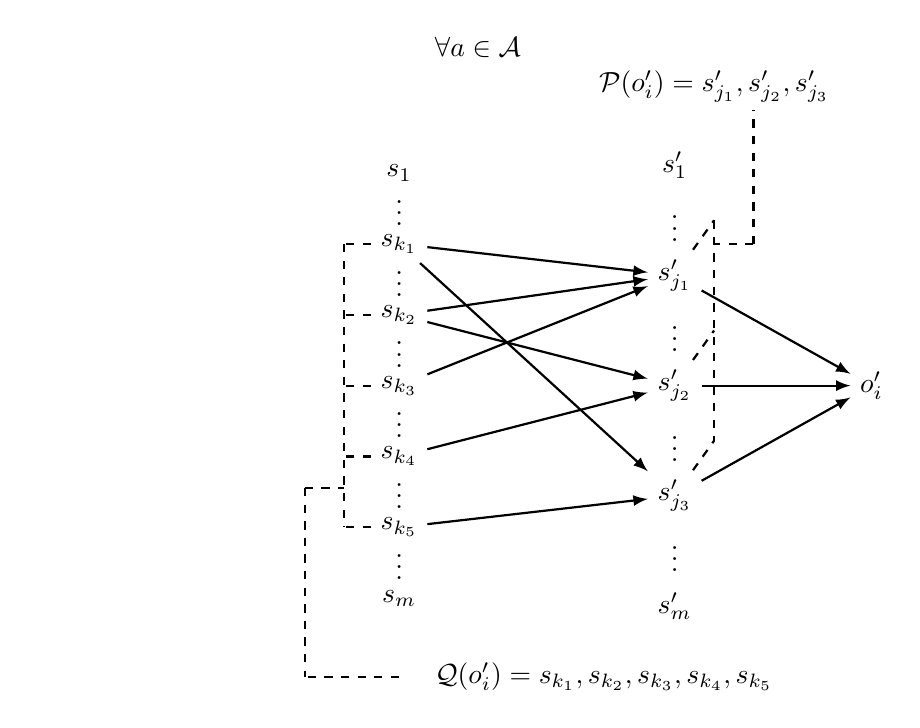
\begin{tikzpicture}
\node (rien) at (-4.6,0) {};
\node (a) at (1,1) {$\forall a \in \mathcal{A}$};
\node (s1) at (0,-0.6) {$s_1$};
\node (dots1) at (0,-1) {$\vdots$};
\node (sk1) at (0,-1.5) {$s_{k_1}$};
\node (dots2) at (0,-1.9) {$\vdots$};
\node (sk2) at (0,-2.4) {$s_{k_2}$};
\node (dots3) at (0,-2.8) {$\vdots$};
\node (sk3) at (0,-3.3) {$s_{k_3}$};
\node (dots4) at (0,-3.7) {$\vdots$};
\node (sk4) at (0,-4.2) {$s_{k_4}$};
\node (dots4) at (0,-4.6) {$\vdots$};
\node (sk5) at (0,-5.1) {$s_{k_5}$};
\node (dots4) at (0,-5.5) {$\vdots$};
\node (sm) at (0,-6) {$s_m$};

\node (sp1) at (3.5,-0.5) {$s_1'$};
\node (dotsp1) at (3.5,-1.2) {$\vdots$};
\node (spj1) at (3.5,-1.9) {$s'_{j_1}$};
\node (dotsp2) at (3.5,-2.6) {$\vdots$};
\node (spj2) at (3.5,-3.3) {$s'_{j_2}$};
\node (dotsp3) at (3.5,-4) {$\vdots$};
\node (spj3) at (3.5,-4.7) {$s'_{j_3}$};
\node (dotsp4) at (3.5,-5.4) {$\vdots$};
\node (smp) at (3.5,-6.1) {$s'_m$};
\draw[->,>=latex,thick] (sk1) to (spj1);
\draw[->,>=latex,thick] (sk2) to (spj1);
\draw[->,>=latex,thick] (sk3) to (spj1);
\draw[->,>=latex,thick] (sk2) to (spj2);
\draw[->,>=latex,thick] (sk4) to (spj2);
\draw[->,>=latex,thick] (sk1) to (spj3);
\draw[->,>=latex,thick] (sk5) to (spj3);
\node (opi) at (6,-3.3) {$o'_{i}$};
\draw[->,>=latex,thick] (spj1) to (opi);
\draw[->,>=latex,thick] (spj2) to (opi);
\draw[->,>=latex,thick] (spj3) to (opi);
\coordinate (sk1bis) at (-0.7,-1.5) {};
\coordinate (sk2bis) at (-0.7,-2.4) {};
\coordinate (sk3bis) at (-0.7,-3.3) {};
\coordinate (sk4bis) at (-0.7,-4.2) {};
\coordinate (sk5bis) at (-0.7,-5.1) {};
\draw[thick,dashed] (sk1) to (sk1bis);
\draw[thick,dashed] (sk2) to (sk2bis);
\draw[thick,dashed] (sk3) to (sk3bis);
\draw[thick,dashed] (sk4) to (sk4bis);
\draw[thick,dashed] (sk5) to (sk5bis);
\draw[thick,dashed] (sk1bis) to (sk5bis);
\node (parents) at (2.6,-7) {$\mathcal{Q}(o_i') = 
\set{ s_{k_1},s_{k_2},s_{k_3},s_{k_4},s_{k_5} }$};
\coordinate (qpa4) at (-0.7,-4.6) {};
\coordinate (qpa3) at (-1.2,-4.6) {};
\coordinate (qpa2) at (-1.2,-7) {};
\coordinate (qpa) at (0,-7) {};
\draw[thick,dashed] (qpa) to (qpa2);
\draw[thick,dashed] (qpa3) to (qpa2);
\draw[thick,dashed] (qpa3) to (qpa4);

\coordinate (h2) at (4,-1.2) {};
\coordinate (m2) at (4,-2.6) {};
\coordinate (b2) at (4,-4) {};
\draw[thick,dashed] (spj1) to (h2);
\draw[thick,dashed] (spj2) to (m2);
\draw[thick,dashed] (spj3) to (b2);
\draw[thick,dashed] (h2) to (b2);
\node (h2) at (4,0.5) {$\mathcal{P}(o_i') = \set{ s'_{j_1}, s'_{j_2}, s'_{j_3} }$};
\coordinate (pa4) at (4,-1.5) {};
\coordinate (pa3) at (4.5,-1.5) {};
\coordinate (pa2) at (4.5,0.2) {};
\draw[thick,dashed] (pa3) to (pa2);
\draw[thick,dashed] (pa3) to (pa4);
\end{tikzpicture}
\caption[Grand-parents of an observation variable]{Whatever the action $a \in \mathcal{A}$, only five state variables 
influence variable $o'_i$ in this Bayesian network: 
$s_{k_1}$, $s_{k_2}$, $s_{k_3}$, $s_{k_4}$, $s_{k_5}$ 
which constitute $\mathcal{Q}(o_i')$.}
\label{obsVarDep}
\end{figure}

Observation probability distributions, knowing previous state variables, 
are then defined $\forall i=1,\ldots,n$
\begin{equation}
\label{obsDistrib} \textbf{p} \paren{ o_i' \sachant \mathcal{Q}(o_i'), a } = \sum_{ v \in 2^{\mathcal{P}(o'_i)}} \textbf{p} \paren{ o'_i \sachant v ,a } \cdot \textbf{p} \paren{ v \sachant \mathcal{Q}(o_i') ,a}
\end{equation}
Therefore a possibilistic belief defined on $2^{ \mathcal{Q}(o_i')}$ is enough to
get the approximate probability distribution of an observation variable, Equation \ref{obsProb}: 
such an epistemic state
leads via transformation \ref{transform} to a probability distribution $\overline{\beta}$
over $2^{\mathcal{Q}(o_i')}$. 
Finally, the approximate probability distribution of the observation variable $i$,
factored counterpart of former equation \ref{obsProb}, is:
\begin{equation}
\label{probObel}
\textbf{p} \paren{ o_i' \sachant \beta,a } = \sum_{ v \in 2^{\mathcal{Q}(o_i')}} \textbf{p} \paren{ o_i' \sachant v,a } \cdot \overline{\beta}(v).
\end{equation}

\subsection{State variables classification}
\label{classif}
State variables $s \in \mathbb{S}$ do not play the same role
in the process: as already studied in the literature \cite{OngShaoHsuWee-IJRR10},
some variables can be visible for the agent, and namely this \textit{mixed-observability}
leads to important computational simplifications. Moreover, some variables do not
affect observation variables, and factorization of the POMDP is then easily transmitted
to the epistemic state based MDP. Finally, using rewrittings of previous sections,
useless computations are highlighted.
\begin{itemize}
\item A state variable $s_j$ is said to be \textbf{visible}, if $\exists o_i \in \mathbb{O}$, 
observation variable, such that $\mathcal{P}(o_i') = \set{ s_j' }$ 
and $\forall a \in \mathcal{A}$, $\textbf{p} \paren{ o_i' \sachant s_j',a } = \mathds{1}_{ \set{o_i' = s_j'}}$
\textit{i.e.} if $o_i' = s_j'$ almost surely. The set of visible state variables is denoted by 
$\mathbb{S}_v = \set{s_{v,1}, s_{v,2}, \ldots, s_{v,m_{v}}}$;
\end{itemize}

Observation variables corresponding to visible state variables can be removed 
from the set of observation variables: the number of observation variables becomes 
$\tilde{n}$, and remaining observation variables are denoted by $o_1,\ldots,o_{\tilde{n}}$.
\begin{itemize}
\item \textbf{Inferred hidden variables} are simply $\cup_{i=1}^{\tilde{n}} \mathcal{P}(o_i')$, 
\textit{i.e.} all hidden variables influencing (remaining) observation variables. The set of
inferred hidden variables is $\mathbb{S}_h = \set{s_{h,1},s_{h,2}, \ldots, s_{h,m_h}}$ and 
contains possibly visible variables.
\item \textbf{Non-inferred hidden variables} or \textbf{fully hidden variables}, denoted by $\mathbb{S}_f$, 
consists of hidden state variables which do not influence any observation, 
\textit{i.e.} all remaining state variables. The fully hidden variables are denoted by 
$s_{f,1},s_{f,2}, \ldots, s_{f,m_f}$, and the corresponding set is $\mathbb{S}_{f}$.
\end{itemize}
Of course, this classification leads to a partition of the initial set of state variables 
if potential visible variables are removed from
inferred hidden variables: denoting purely inferred hidden variables by $\overline{\mathbb{S}}_h = \mathbb{S}_h \setminus \mathbb{S}_v$, 
and $\overline{m}_h = \# \overline{\mathbb{S}}_h$ the state variables partition is 
$\mathbb{S} = \mathbb{S}_v \sqcup \overline{\mathbb{S}}_h \sqcup \mathbb{S}_f$ and $m = m_v + \overline{m}_h + m_f$.

The classification defined here is used to avoid some computations for visible variables:
if $s_{v} \in \mathbb{S}_v$ is visible, and $o_{v} \in \mathbb{O}$ is the associated observation ($s_v=o_v$ almost surely), 
computations of the distribution over $\mathcal{P}(o'_v)$, Equation \ref{distribPOP}, and
of the distribution over $o'_v$, Equation \ref{obsDistrib}, are unnecessary: the distribution 
over $s'_v$ $(=o'_v)$ needed is simply given by $\textbf{p} \paren{ s'_v \sachant \mathcal{P}(s'_v), a } $, 
data of the original problem. The counterpart of Equation \ref{probObel} is then
\begin{equation}
\label{probSVbel}
\textbf{p} \paren{ s'_v \sachant \beta, a } = \sum_{2^{\mathcal{P}(s'_v)}} \textbf{p} \paren{ s'_v \sachant \mathcal{P}(s'_v), a } \cdot \overline{\beta}(\mathcal{P}(s'_v)),
\end{equation}
where $\overline{\beta}$ is the probability distribution over $2^{\mathcal{P}(s'_v)}$ 
extracted from the possibilistic belief over the same space, using transformation (\ref{transform}).
\subsection{Joint possibility distributions}
%In this work, beliefs, or epistemic states of the agent, are reduced to
%fuzzy sets of possible system states (instead of classical probability distributions $b: \mathcal{S} \rightarrow [0,1]$). 
%Such successive beliefs are built using 
Possibility distributions of the problem are here
nothing more than probability distributions previously defined, normalized 
in a possibilistic sense: if $v \in \set{\top,\bot}$ maximizes $\textbf{p}(v)$,
$\pi(v)=1$, otherwise $\pi(v)=\textbf{p}(v)$.

Joint possibility distributions over $o_i' \times \mathcal{P}(o'_i)$, needed for belief process definition (possibilistic belief update, Theorem \ref{belief_process_recursif_poss}), 
are computed in the following way:
\begin{eqnarray*}
\pi \paren{ o_i', \mathcal{P}(o'_i) \sachant \mathcal{Q}(o'_i), a } & = & \min \set{ \pi \paren{ o_i' \sachant \mathcal{P}(o'_i), a}, \pi \paren{ \mathcal{P}(o'_i) \sachant \mathcal{Q}(o'_i), a  } } \\
& = & \min \set{ \pi \paren{ o_i' \sachant \mathcal{P}(o'_i), a}, \min_{s'_j \in \mathcal{P}(o'_i)} \pi \paren{ s'_j \sachant \mathcal{P}(s'_j), a  } }.
\end{eqnarray*}

%\nico{
%Recall the possibilistic Bayes rule: $b^{a,o'}(s')$
%\[  =  
%\left \{  \begin{array}{cc} 
%1 & \mbox{ if }  \pi \paren{ o', s' \sachant b, a } \mbox{ maximizes; } \\
%\pi \paren{ o', s' \sachant b, a } & \mbox{ otherwise }. 
% \end{array}  \right .
%\]

%This Bayes rules can be decomposed into two step:

%\textbf{joint distribution computation: } 
%\begin{equation}
%\pi \paren{ o', s' \sachant b, a } = \min \set{ \pi \paren{ o',s' \sachant s,a} , b(s) } \\
%\end{equation}
%\textbf{possibilistic normalization}:
%\begin{eqnarray}
%\mbox{ if } s' \in argmax_{s'} \pi \paren{ o', s' \sachant b, a }, \\
%\nonumber \mbox{ then } \pi \paren{ o', s' \sachant b, a } = 1.
%\end{eqnarray}
%}
\subsection{Beliefs process definition and handling}
This section is meant to define marginal belief distributions instead of a global one,
in order to benefit from the factorized structure of the initial POMDP. Indeed,
possibilistic belief distributions have different definitions according to which class of state variables they concern:
\begin{itemize}
\item as visible state variables are directly observed, there is no uncertainty over
 these variables. Two epistemic states (possibilistic belief distribution) 
are possible for visible state variable 
$s'_{v,j}$: 
$b_{v,T}'(s'_{v,j}) = \mathds{1}_{ \set{s'_{v,j}=\top}}$ and 
$b_{v,F}'(s'_{v,j}) = \mathds{1}_{\set{s'_{v,j}=\bot}}$. As a consequence, one boolean variable 
$\beta_{v,j}' \in \set{ \top, \bot }$ per visible state variables is enough to represent this 
belief distribution in practice: if $s'_{v,j}=\top$, then next belief is $b'=b_{v,T}'$ represented 
by belief variable assignment $\beta'_{v,j} = \top$, otherwise, next belief is $b'=b_{v,F}'$, and $\beta'_{v,j} = \bot$.
A belief variable of a visible state variable is denoted by $\beta_v$.
%Finally, a visible state variable $s_v$ and its associated belief variable $\beta_v$ are confused,
%Visible state variables are then confused with the belief one ???($s_{v,j}=b_{v,j}$). 
\item for each $i \in 1,\ldots,\tilde{n}$, each inferred hidden variable constituting 
$\mathcal{P}(o'_i)$ is an input of the same possibilistic belief distribution: 
non-normalized belief is, $\forall i=1,\ldots,\tilde{n}$
\end{itemize}
\begin{equation}
\label{inferredBel}
\tilde{b}'(\mathcal{P}(o_i')) = \max_{v \in 2^{\mathcal{Q}(o_i')}} \min \set{ \pi \paren{ o_i', \mathcal{P}(o_i') \sachant v,a}, b(v) }.
\end{equation}
A possibilistic normalization finalizes the belief update: for $w \in 2^{\mathcal{P}(o_i')}$,
\begin{eqnarray}
\label{possNorm} b'(w') & = & \left \{ \begin{array}{ccc} 1 \mbox{ if } w' \in \operatorname*{argmax}_{v' \in 2^{\mathcal{P}(o_i')}} \tilde{b}'(v'); \\
 \tilde{b}'(w') \mbox{ otherwise} . \end{array} \right.
\end{eqnarray} 
In practice, if $l=\# \mathcal{L}$ is the size of the possibility scale, and $p_i = \# \mathcal{P}(o_i')$, the number of belief states
is $l^{2^{p_i}} - (l-1)^{2^{p_i}}$, and then the number of belief variables is $n_{h,i} = \lceil \log_2(l^{2^{p_i}} - (l-1)^{2^{p_i}}) \rceil$.
A belief variable of an inferred hidden state variable is denoted by $\beta_h$.
\begin{itemize}
\item for each $j \in 1,\ldots,m_f$, non-normalized belief defined on fully hidden 
variable $s_{f,j}$ is 
\end{itemize}
\begin{equation}
\label{fullyHiddenBel}
\tilde{b}'(s_{f,j}') = \max_{v \in 2^{\mathcal{P}(s_{f,j}') }} \min \set{ \pi \paren{ s_{f,j}' \sachant v,a}, b(v) },
\end{equation}
which leads to the actual new belief $b'$ after normalization (\ref{possNorm}).
In practice, as each fully hidden variable is considered independently from the others, 
following the previous reasoning for vector of inferred hidden s.v., 
the number of belief variables is $n_f = \lceil \log_2(l^2 - (l-1)^2) \rceil = \lceil \log_2(2l-1) \rceil$.
A belief variable of a fully hidden state variable is denoted by $\beta_f$. \\

Finally the actual global epistemic state $b'(\mathbb{S}')$ is upper bounded by 
\begin{equation}
b'(\mathbb{S}') = \min \set{ \min_{j=1}^{m_v} b'(s'_{v,j}), \min_{i=1}^{\tilde{n}} b'(\mathcal{P}(o_i')), \min_{k=1}^{m_f} b'(s_{f,k}') },
\end{equation}
where $\mathbb{S}$ has to be seen as a vector composed of all state variables.\\
The latter is considered as the agent belief
to make the final MDP factorized.

\subsection{Select and use belief variables}
Starting with initial beliefs defined for each visible state variable $s_{v,j}$,
for each vector of inferred hidden variables $\mathcal{P}(o'_i)$ and for each fully 
hidden variable $s_{f,j}$, these beliefs are updated at each time step according to the
transformations described above.

However previous formulae \ref{inferredBel} 
and distribution over observation variable $o'_i \in \mathbb{O}$, Equation \ref{probObel}, 
depend on belief distribution
over $\mathcal{Q}(o'_i) \subseteq \mathbb{S}$.
They can be computed from the available beliefs as follow: $\forall i=1,\ldots,\tilde{n}$,
\begin{eqnarray}
\label{bq}
b(\mathcal{Q}(o_i')) = \max_{v \in 2^{\mathcal{K}_i}}  \min \set{ \min_{s_{v} \in \mathcal{Q}(o_i') \cap \mathbb{S}_v} b(s_{v}), \min_{j \in \mathcal{J}_i }  b(\mathcal{P}(o_j)), \min_{s_{f} \in \mathcal{Q}(o_i') \cap \mathbb{S}_f} b(s_{f}) },
\end{eqnarray}
where
\begin{itemize}
\item $\mathcal{J}_i = \set{ j \in \set{1,\ldots,\tilde{n}} \mbox{ s.t. } \mathcal{P}(o_j) \cap \mathcal{Q}(o_i') \neq \emptyset}$, \textit{i.e.} $\mathcal{J}_i$ is the set of indices $j$ 
for which $\mathcal{P}(o_j)$ shares (inferred hidden) state variables with $\mathcal{Q}(o_i')$,
and
\item $\mathcal{K}_i = \set{\cup_{j \in \mathcal{J}_i} \mathcal{P}(o_j)} \setminus \mathcal{Q}(o_i') \subseteq \mathbb{S}_h$, \textit{i.e.} $\mathcal{K}_i$ 
is the set of (inferred hidden) state variables which are not present in 
$\mathcal{Q}(o_i')$, but are present in a set $\mathcal{P}(o_j)$ 
sharing state variables with $\mathcal{Q}(o_i')$. 
\end{itemize}
As well, belief update for fully hidden state variables, Equation \ref{fullyHiddenBel}, 
needs a belief distribution over variables $\mathcal{P}(s_{f,j}')$:
$\forall j=1,\ldots,m_f$, 
\begin{eqnarray} 
\label{bp}
b(\mathcal{P}(s_{f,j}')) =  \max_{v \in 2^{\mathcal{N}_j}}  \min \set{ \min_{s_{v} \in \mathcal{P}(s_{f,j}') \cap \mathbb{S}_v} b(s_{v}),
\nonumber\min_{k \in \mathcal{M}_j }  b(\mathcal{P}(o_k)), \min_{s_{f} \in \mathcal{P}(s_{f,j}') \cap \mathbb{S}_f} b(s_{f}) },
\end{eqnarray}
where
\begin{itemize}
\item $\mathcal{M}_j= \set{ k \in \set{1,\ldots,m_f} \mbox{ s.t. } 
\mathcal{P}(o_k) \cap \mathcal{P}(s_{f,j}') \neq \emptyset}$, \textit{i.e.} $\mathcal{M}_j$ 
is the set of indices $k$ for which $\mathcal{P}(o_k)$ shares (inferred hidden) state variables with $\mathcal{P}(s_{f,j}')$, and
\item $\mathcal{N}_j = \set{\cup_{k \in \mathcal{M}_j} \mathcal{P}(o_k)} 
\setminus \mathcal{P}(s_{f,j}') \subseteq \mathbb{S}_h$, \textit{i.e.} $\mathcal{N}_j$ 
is the set of (inferred hidden) state variables which are not present in 
$\mathcal{P}(s_{f,j}')$, but are present in a set $\mathcal{P}(o_k)$ 
sharing state variables with $\mathcal{P}(s_{f,j}')$. 
\end{itemize}
Finally, a belief distribution over $\mathcal{P}(s_{v,i}')$ needed to define an
approximate probability distribution over visible state variables (Equation \ref{probSVbel}),
can be defined in the same way, marginalizing ($\max$) over unused variables.

\section{Solving a POMDP with a discrete MDP solver}
The previous section leads to a factored MDP, whose the version used in practice is defined here.
A concrete POMDP problem and its resulting MDP are then described in order to highlight
the power in state space size reduction of the possibilistic structured translation.
%This problem is then tested as an input of the solver PROST, and compared to POMDP solvers.
%PROST \cite{conf/aips/KellerE12} is a state-of-the-art finite horizon and discrete MDP solver:
%it won the two last discrete probabilistic planning competition \cite{SannerIPPC11}.
\subsection{Resulting factored MDP:}
Section \ref{classif} classifies state variables in order to define epistemic states $b$
over sets of state variables (respectively $\forall j=1,\ldots,m_v$, $\set{s^v_j}$, 
$\forall i=1,\ldots,\tilde{n}$, $\mathcal{P}(o'_i)$, and $\forall k=1,\ldots,m_f$, 
$\set{ s^f_j }$) and set of variables encoding them (respectively $\beta_v$, $\beta_h$ and  
$\beta_f$) independently to each other. As belief updates are deterministic knowing the
observation, a simple trick is used to keep this determinism in the final MDP:
a $flipflop$ boolean variable is introduced, changing its state at each step, denoted
by $f$. It
artificially divides a classical time step of the POMDP into two phases.
During the first phase, called \textit{the observation generation phase}, 
non-identity transition functions 
(\textit{i.e.} which do not let the variable remain the same)
are the probability distributions over observation variables \ref{probObel}
and visible state variables \ref{probSVbel}.

During the second phase, called \textit{the belief update phase}, 
non-identity transition functions are
the deterministic transitions of the belief variables:
\begin{itemize}
\item variable $\beta_v$ is updated knowing value of the corresponding visible variable $s_v$;
\item variables $\beta^{1}_{h}, \ldots, \beta^{n_{h,i}}_h$ are updated knowing value of observation variable $o_i$, 
and using update \ref{inferredBel}, \ref{possNorm};
\item variables $\beta^{1}_{f}, \ldots, \beta^{n_{f}}_f$ using update \ref{fullyHiddenBel}.
\end{itemize}

The state space is then defined as:  \\
$\mathcal{S} = f \times s^1_v \times \ldots \times s^{m_v}_v 
\times o^1 \times \ldots \times o^{\tilde{n}}  \times \beta^1_v \times \ldots 
\times \beta^{m_v}_v \times \beta^1_h  \times \ldots \times \beta^{\tilde{n}}_h 
\times \beta^1_f \times \ldots \times \beta^{m_f}_f $, where $\forall i=1,\ldots,\tilde{n}$, 
$\beta^i_h$ represents boolean variables $\beta^{1,i}_{h}, \ldots, \beta^{n_{h,i},i}_h$, and
$\forall k=1,\ldots,m_f$, $\beta^{j}_f$ represents boolean variables $\beta^{1,j}_{f}, \ldots, \beta^{n_{f},j}_f$.

\begin{figure}\centering
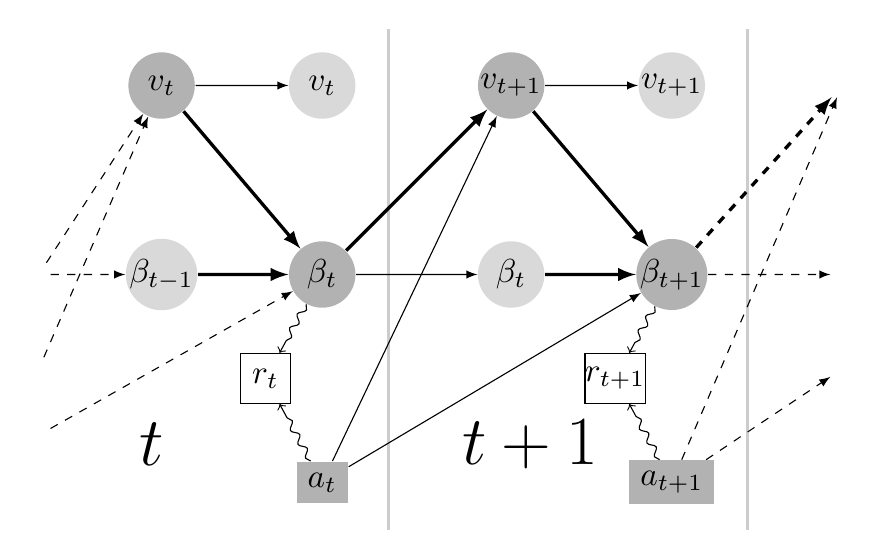
\begin{tikzpicture}[scale=1.2,transform shape]

%TIME/BACKGROUND
\coordinate (middleTop) at (5.7,3.6);
\coordinate (middleBot) at (5.7,-1.7);
\draw[thick,color=black!20] (middleTop) -- (middleBot);
\node [font=\huge] (statet) at (3.2,-0.8) {$t$};
\coordinate (middleTop2) at (9.5,3.6);
\coordinate (middleBot2) at (9.5,-1.7);
\draw[thick,color=black!20] (middleTop2) -- (middleBot2);
\node [font=\huge] (statetplus1) at (7.2,-0.8) {$t+1$};

%%%%%%%%%%%%%%%%%%%%%%%%%%%%%%%%%%%%%%%%%%%%%%%%%%%%%%%%%%%%%%
%vertex
%vars
\tikzstyle{vertex}=[circle,fill=black!30,minimum size=20pt,inner sep=0pt]
\tikzstyle{vertex2}=[circle,fill=black!15,minimum size=20pt,inner sep=0pt]
%r
\tikzstyle{vertex3}=[ draw, inner sep=0pt, minimum size=15pt]

%1
\node[vertex] (state1) at (3.3,3) {$v_t$};
%\node[vertex] (state13) at (3.3,2) {$s^v_{t}$};
\node[vertex2] (state12) at (3.3,1) {$\beta_{t-1}$};
%1bis
\node[vertex2] (state1bis) at (5,3) {$v_t$};
%\node[vertex2] (state13bis) at (5,2) {$s^v_{t}$};
\node[vertex] (state12bis) at (5,1) {$\beta_t$};
%R1
\node[vertex3] (R1) at (4.4,-0.1) {$r_t$};

%2
\node[vertex] (state2) at (7,3) {$v_{t+1}$};
%\node[vertex] (state23) at (7,2) {$s^v_{t+1}$};
\node[vertex2] (state22) at (7,1) {$\beta_{t}$};

%2bis
\node[vertex2] (state2bis) at (8.7,3) {$v_{t+1}$};
%\node[vertex2] (state23bis) at (8.7,2) {$s^v_{t+1}$};
\node[vertex] (state22bis) at (8.7,1) {$\beta_{t+1}$};
%R2
\node[vertex3] (R2) at (8.1,-0.1) {$r_{t+1}$};

%0
\node (state02) at (2,1) {};
\node (state03) at (2,2) {};
%3
\node (state3) at (10.5,3) {};
\node (state33) at (10.5,2) {};
\node (state32) at (10.5,1) {};

\node (state32bis) at (10.5,0) {};

%action
\node[fill=black!30] (action) at (5,-1.2) {$a_t$};
\node (action0) at (2,0) {};
\node (action02) at (2,-0.7) {};
\node[fill=black!30] (action3) at (8.7,-1.2) {$a_{t+1}$};

%%%%%%%%%%%%%%%%%%%%%%%%%%%%%%%%%%%%%%%%%%%%%%%%%%%%%%%%%%%%%%
%ARROWS

%1->2
\draw[->,>=latex] (state1) -- (state1bis);
\draw[->,>=latex,very thick] (state1) -- (state12bis);
\draw[->,>=latex, very thick] (state12) -- (state12bis);
%\draw[->,>=latex] (state13) -- (state13bis);
%1->2bis
\draw[->,>=latex, very thick] (state12bis) -- (state2);
\draw[->,>=latex] (state12bis) -- (state22);
%\draw[->,>=latex, very thick] (state13bis) -- (state2);
%\draw[->,>=latex, very thick] (state13bis) -- (state23);
%\draw[->,>=latex, very thick] (state12bis) -- (state23);
%\draw[->,>=latex, very thick, color=red] (state13bis) -- (state22);
%0->1
\draw[->,>=latex,dashed] (state02) -- (state1);
\draw[->,>=latex,dashed] (state02) -- (state12);
%\draw[->,>=latex,dashed] (state02) -- (state13);
%\draw[->,>=latex,dashed] (state03) -- (state13);
%2->3
\draw[->,>=latex] (state2) -- (state2bis);
\draw[->,>=latex, very thick] (state2) -- (state22bis);
\draw[->,>=latex, very thick] (state22) -- (state22bis);
%\draw[->,>=latex] (state23) -- (state23bis);
%2->3bis
\draw[->,>=latex,dashed, very thick] (state22bis) -- (state3);
\draw[->,>=latex,dashed] (state22bis) -- (state32);
%\draw[->,>=latex,dashed, very thick] (state22bis) -- (state33);
%\draw[->,>=latex,dashed, very thick] (state23bis) -- (state33);
%\draw[->,>=latex,dashed, very thick] (state23bis) -- (state3);
%\draw[->,>=latex,dashed, very thick, color=red] (state23bis) -- (state32);
%action
%1
\draw[->,>=latex] (action) -- (state2);
\draw[->,>=latex] (action) -- (state22bis);
%\draw[->,>=latex] (action) -- (state23);
\draw[->,decorate,decoration={snake,amplitude=.4mm,segment length=2mm,post length=1mm}] (action) -- (R1); 
%0
\draw[->,>=latex,dashed] (action0) -- (state1);
%\draw[->,>=latex,dashed] (action0) -- (state13);
\draw[->,>=latex,dashed] (action02) -- (state12bis);
%3
\draw[->,>=latex,dashed] (action3) -- (state3);
%\draw[->,>=latex,dashed] (action3) -- (state33);
\draw[->,>=latex,dashed] (action3) -- (state32bis);
\draw[->,decorate,decoration={snake,amplitude=.4mm,segment length=2mm,post length=1mm}] (action3) -- (R2); 

% R
\draw[->,decorate,decoration={snake,amplitude=.4mm,segment length=2mm,post length=1mm}] (state12bis) -- (R1); 
%\draw[->,decorate,decoration={snake,amplitude=.4mm,segment length=2mm,post length=1mm}] (state1) -- (R1); 
\draw[->,decorate,decoration={snake,amplitude=.4mm,segment length=2mm,post length=1mm}] (state22bis) -- (R2); 
%\draw[->,decorate,decoration={snake,amplitude=.4mm,segment length=2mm,post length=1mm}] (state2) -- (R2); 
\end{tikzpicture}
\caption[Practical DBN of the resulting MDP]{Practical DBN of the resulting MDP: thickest arrows illustrate transitions which are not
identity transitions.}
\label{DBN}
\end{figure}

The resulting MDP is illustrated in Figure \ref{DBN} where $\beta_t$ represents all belief variables,
and $v_t$ the visible variables: flipflop variable $f$, observations $o_i$ and visible state variables $s_v$.

This trick makes the belief update phase deterministic. Each belief variable
transition can be then deterministically defined, and independently from
each other: as visible state and observation variables are already post-action independent, 
the resulting MDP is a factored MDP.
\subsection{Results for a concrete POMDP problem}
A problem inspired by the RockSample problem \cite{Smith:2004:HSV:1036843.1036906} is described in this section
to illustrate the factorized possibilistic discretization of the agent belief, from a factored POMDP:
a rover is navigating in a place described by a finite number of locations $l_1, \ldots, l_n$,
and where stand $m$ rocks. Some of these $m$ rocks have an interest in the scientific
mission of the rover, and it has to sample them. However, sampling a rock is an expensive
operation. The rover is thus fitted with a long range sensor making him able to estimate if
the rock has to be sampled. Finally operating time of the rover is limited, but its battery
level is available.

Variables of this problem can now be set, and classified as in Section \ref{classif}:
as the battery level is directly observable by the agent (the rover), the set of
visible state variables consists of the boolean variables encoding it: $\mathbb{S}_v = \set{B_1, B_2, \ldots, B_k}$.
The agent knows the different locations of the rocks, however the nature of a rock is estimated.
The set of inferred hidden state variables consists of $m$ boolean variables $R_i$ encoding the nature
of the $i^{th}$ rock, $\top$ for ``scientifically good'' and $\bot$ otherwise: 
$\mathbb{S}_h = \set{R_1, R_2, \ldots, R_m}$. When the $i^{th}$ rock is observed using the sensor, it returns a noisy 
observation of the rock in $\set{\top,\bot}$, modeled by the boolean variable $O_i$: the set of observation
variables is then $\mathbb{O} = \set{O_1, O_2, \ldots, O_m}$.
Finally, no localization equipment is provided: the agent estimates its location from its initial information,
and its dynamics. Each location of the rover is formally described by a variable $L_j$, which equals $\top$
if the rover is at the $j^{th}$ location, and $\bot$ otherwise. The set of fully hidden variables consists thus
of these $n$ variables: $\mathbb{S}_f = \set{L_1, L_2, \ldots, L_{n}}$. 

Initial location is known, described by variable $L_1$, and leading to a deterministic initial belief: 
$\beta_0(\mathcal{S}_h) = 1$ if $L_1=\top$ and $L_j = \bot$ $\forall j \neq 1$, $0$ otherwise. However
initial nature of each rock is not known. Instead of a uniform probability distribution over the
rocks nature (``rock has to be sampled'', or ``rock is not interesting''), the Possibility Theory allows to represent this initial ignorance with the
marginal belief $\beta_0(\mathcal{S}_h) = 1$, for each assignment of the hidden inferred state variables
modelling nature of the rocks. 

Finally, the factorization trick leads to a reduction of the domain size: 
with a flat translation of this POMDP, the size of the resulting state space is described with
$\lceil \log_2( \# \mathcal{L}^{2^{n+m+k}} - (\# \mathcal{L}-1)^{2^{n+m+k}}) \rceil$ boolean variables.
Taking advantage of the POMDP structure, the resulting state space is encoded with 
$1+2 \cdots k+m+(m+n).\lceil \log_2(2 \# \mathcal{L} -1 )  \rceil$ Boolean variables:
the flipflop variable, the visible variables and associated beliefs variables, 
the observation variables, and the belief variables 
associated to the fully hidden and inferred hidden variables.

Moreover, the dynamic of the resulting MDP is factorized: all variables are independent post-action,
and lots of them are deterministic, thank to the flipflop variable trick.
These structures are beneficial to the MDP solvers,
leading to faster computations.

%preprocessing with ADDs \cite{Bahar:1997:ADD}
%\cite{SannerIPPC11}
\section{Conclusion}
This chapter described a hydrid translation 
of a POMDP problem into a finite state space MDP one:  
the Qualitative Possibility Theory, 
is used here to maintain an epistemic state during the process. 
The MDP problem, result of this translation, 
is entirely built defining transition and reward functions
over these epistemic states. 
Definitions of these functions use respectively the pignistic transformation,
used to recover a probability distribution 
from an epistemic state, 
and the Choquet integral with respect to the necessity, 
making the agent pessimistic about the potential ignorance 
described by its epistemic state.
A practical way to implement this translation 
is then described: 
with these computations, 
a factored POMDP leads to a factored and tractable MDP problem. 
The essential particularity of this translation 
is the granular modeling of the agent belief 
using a qualitative fuzzy knowledge representation 
Finally this promising approach will be tested on RDDL files 
of the IPPC competition \cite{SannerIPPC1111}
using a state of the art MDP planner like PROST 
\cite{conf/aips/KellerE12}. Indeed these files describe
factored POMDP problems as introduced in Section \ref{factorizationSection}.
